\documentclass[11pt,a4paper]{article}

\usepackage[utf8]{inputenc}
\usepackage[T1]{fontenc}
\usepackage[margin=2.5cm]{geometry}
% \usepackage[demo]{graphicx}
\usepackage{graphicx}
\graphicspath{{images/}}
\usepackage{booktabs}
\usepackage{float}
\usepackage{hyperref}
\usepackage{caption}
\usepackage{subcaption}
\usepackage{enumitem}
\usepackage{amsmath}

\hypersetup{
    colorlinks=true,
    linkcolor=black,
    citecolor=black,
    urlcolor=blue
}

\title{
    Application Project SoSe 26\\
    \vspace{0.4em}
    \textbf{Group 2: TKMS - CV Maritime Navigation}
}

\author{
    Nur Bozdemir \and
    Meliona Meliona \and
    Tim Prause
}

\date{\today}

\begin{document}

\begin{titlepage}
    \centering

    {\Large Application Project SoSe 26\par}
    \vspace{0.5cm}

    {\Huge\bfseries Group 2: TKMS - CV Maritime Navigation\par}
    \vspace{0.7cm}

    {\Large Project Report\par}
    \vspace{2cm}

    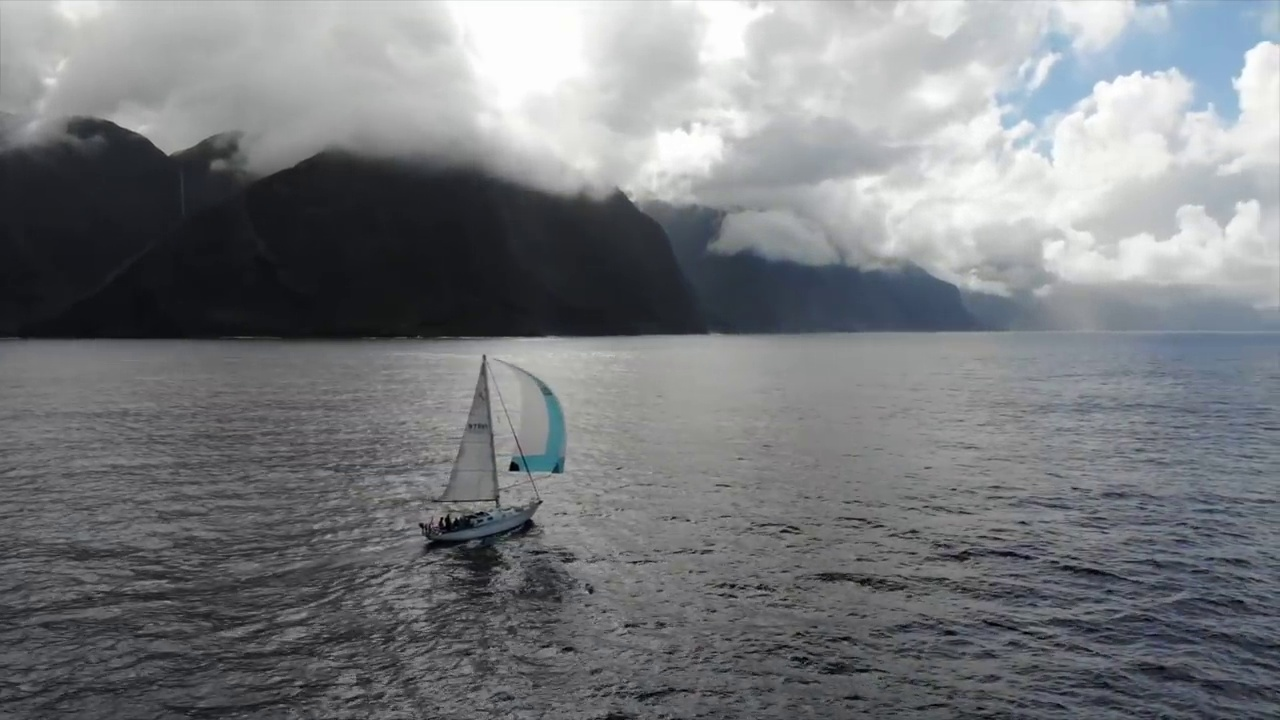
\includegraphics[width=\textwidth]{yt015_03_00049.jpg}

    \vspace{2cm}

    {\large
    Nur Bozdemir\\
    Meliona Meliona\\
    Tim Prause
    \par}

    \vspace{0.5cm}
    {\large \today\par}
\end{titlepage}

\pagenumbering{roman}
\tableofcontents
\clearpage

\pagenumbering{arabic}

% Target length: maximum 30 pages including figures and tables.
% Suggested allocation:
% Abstract 0.5p, Introduction/Data/Goal 3-4p, Methods 8-10p,
% Results 8-10p, Discussion/Limitations/Conclusion/Future Work 5-7p.

\begin{abstract}
Unmanned surface vehicles (USVs) need a reliable vision system to detect
obstacles on the open water. In this application project we study maritime obstacle detection on the LaRS dataset
and benchmark three object detectors from different families: YOLOv8 (one-stage
CNN), Faster R-CNN (two-stage CNN), and RF-DETR (a transformer detector). LaRS
only provides instance masks for its train and validation splits, and we derive the
bounding boxes from the extent of those masks. Several distinct objects sometimes
share a single segment, which produces one oversized box spanning all of them
instead of a separate box per object. We apply a model-assisted cross-validation
relabeling step to clean these cases. We compare
the models on detection accuracy and inference speed, analyse their errors by
object size and class, and apply explainable-AI methods to see where the models
look. RF-DETR gives the best accuracy while still running in real time, and the
live-video test supports this recommendation. The main remaining challenge is
detecting very small objects, and label quality turns out to be the dominant
factor on the measured scores.
\end{abstract}

\section{Introduction}

\subsection{Problem Context}
% TODO: Maritime navigation and USV obstacle detection context.
An Unmanned Surface Vehicle (USV) is a boat that drives itself, without a
person on board. To do this safely, it needs to ``see'' what is around it. It
must find other boats, buoys, swimmers, and other objects on the water to navigate around them savely.

Seeing the water comes with different challenges than seeing a road. A road is flat and stable. The
water surface moves all the time. The sun creates bright reflections, waves can
look like real objects, and small obstacles can be hidden between the waves.
A good vision system has to deal with all of these problems.

\subsection{Project Motivation}
% TODO: Safety, autonomy, real-time perception, maritime edge cases.
Safety is the main reason for this work. If the USV does not see an obstacle in
time, it can crash. This is dangerous for people in the water and for other
boats, and it can damage the vehicle.

The vision system also has to be fast. The boat keeps moving while it looks at
the scene, so it must detect objects in real time. At the same time it has to be accurate, even in hard conditions like glare, fog, or
waves. This project looks for a good balance between speed and accuracy.

\subsection{Problem Statement}
% TODO: Object detection task and target obstacle categories.
We treat the task as object detection. For each image, the model has to draw a
box around every object and say which class it belongs to. We focus on the
maritime classes that matter for safe navigation: boats and ships, row boats,
paddle boards, buoys, swimmers, animals, floats, and other surface obstacles.

\subsection{Goals And Research Questions}
% TODO: Detection performance, speed/accuracy tradeoff, failure modes, XAI.
The goal of this project is to compare different detection models and find out
which one fits a USV best. We train and benchmark several model families,
from proven baselines to newer architectures, on the same data.

We focus on these questions:
\begin{itemize}[noitemsep]
    \item How accurate is each model at detecting maritime objects?
    \item How do the models trade off speed against accuracy?
    \item Where do the models fail, and on which classes or conditions?
    \item When a model makes a decision, what part of the image is it really
          looking at? Is it the object, or the reflection in the water, or something unrelated?
\end{itemize}
The last question is why we also apply Explainable AI (XAI) methods. We do not only want the boxes, we want to understand how the model reaches its decision.

\subsection{Report Structure}
% TODO: Short overview of report sections.
The rest of this report is organized as follows. Section~2 describes the LaRS
dataset and the target classes. Section~3 explains our methods, including
preprocessing, the model architectures, the training setup, and the evaluation
and XAI methodology. Section~4 presents the results. Section~5 discusses what
the results mean for maritime navigation. Section~6 lists the limitations of our
work, and the final sections give the conclusion and ideas for future work.

\section{Data Description}

\subsection{LaRS Dataset Overview}
% TODO: Dataset source, raw splits, image-level and panoptic annotations.
We use the LaRS (Lakes, Rivers and Seas) dataset~\cite{zust2023lars}, one of the first public benchmark for maritime panoptic obstacle detection. It is larger and more diverse than earlier maritime datasets in terms of recording locations, scene types, obstacle classes, and acquisition conditions. The scenes come from three sources: public online videos from around the world, new recordings made by the authors, and the hardest scenes taken from existing maritime datasets.

The dataset contains 4,006 labelled key frames. Each key frame also comes with
the nine frames before it, which gives over 40k frames in total and allows
methods to use temporal information. Figure~\ref{fig:data_samples} shows frames
from one such sequence with their ground-truth boxes. Every key frame has per-pixel panoptic
labels for 3 stuff classes and 8 thing classes, plus 19 global scene attributes
that describe the environment, lighting, reflections, surface roughness, and
special conditions. The original splits are train (65\%), validation (5\%), and
test (30\%). The splits share no sequence, so frames from the same video stay in
one split, and the test labels are kept private behind an online evaluation
server.

In this project we use LaRS v1.0.0. Panoptic masks are available for the train
and validation splits (2,605 and 198 images); the original test split (1,203
images) has image-level labels only. Our task is object detection, so we convert
the panoptic instance masks into bounding boxes.

\subsection{Target Classes}
% TODO: Boat/ship, Row boats, Paddle board, Buoy, Swimmer, Animal, Float, Other.
We detect the 8 classes of the LaRS dataset: boat/ship, row boat,
paddle board, buoy, swimmer, animal, float, and an open-world ``other'' class
for the remaining obstacles. The 3 stuff classes (water, sky, and static
obstacles such as shores and piers) describe the background and are not used as
detection targets.

\subsection{Processed Detection Splits}
% TODO: Train, validation, test, and unused original test split.
An important point is that we \emph{don't} use the original LaRS splits. The
official test set has no instance masks and its labels are withheld behind the
online server, so we cannot use it for detection training or evaluation. We
therefore re-split the labelled data ourselves. We divide the original train
split into our own train (80\%) and test (20\%) sets and keep the original
validation split as our validation set. The original test split is set aside as
an unused split, since it only has image-level labels. The split is done at the
scene level and stratified by scene attributes; the exact procedure is described
in Section~\ref{sec:scene_split}. The resulting splits and their bounding-box
counts are shown in Table~\ref{tab:data_splits}.

\begin{table}[H]
    \centering
    \caption{Overview of processed dataset splits. Box counts are after the
    cross-validation relabeling step (Section~\ref{sec:relabel}).}
    \label{tab:data_splits}
    \begin{tabular}{lrrl}
        \toprule
        Split & Images & Boxes & Notes \\
        \midrule
        Train & 2,102 & 8,025 & 80\% scene-level split of raw train \\
        Validation & 198 & 1,119 & Raw LaRS validation split \\
        Test & 503 & 1,605 & 20\% scene-level split of raw train \\
        Test unused & 1,203 & -- & Image-level labels only \\
        \bottomrule
    \end{tabular}
\end{table}

\subsection{Dataset Characteristics}
% TODO: Scene types, lighting, reflections, waves, class imbalance.
The dataset is visually diverse but also hard for detection. The scenes range from large ports with hundreds of ships in them, to scenes in the arctic with only two research ships. Three properties
stand out from our exploratory analysis of the train and validation splits.

First, the classes are strongly imbalanced. Boat/ship makes up about 64\% of all
instances, while float is the rarest class with only 26 instances (0.2\%). The
ratio between the most and least common class is about 258 to 1. Such imbalance
makes the rare classes much harder to learn.

Second, many objects are small. Bounding-box areas reach down to a single pixel,
and small obstacles like buoys, swimmers, and animals are common (see
Figure~\ref{fig:object_size}). Small objects are a known weak point for detectors
and a key safety concern for a USV.

Third, the scenes contain many difficult conditions. The images cover river-,
sea-, and lake-like environments under different lighting, and they include
challenging effects such as strong reflections, sun glitter, fog, rain, wakes,
and plants or debris on the water. These are exactly the conditions where a
model can confuse the real object with its reflection.

\begin{figure}[H]
    \centering
    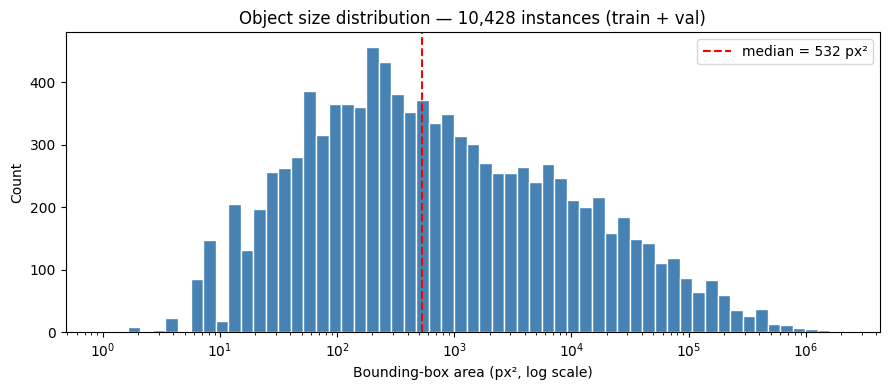
\includegraphics[width=0.8\textwidth]{object_size.png}
    \caption{Distribution of bounding-box areas (log scale) for all object
    instances. Many objects are very small.}
    \label{fig:object_size}
\end{figure}

\begin{figure}[H]
    \centering
    \begin{subfigure}{0.32\textwidth}
        \centering
        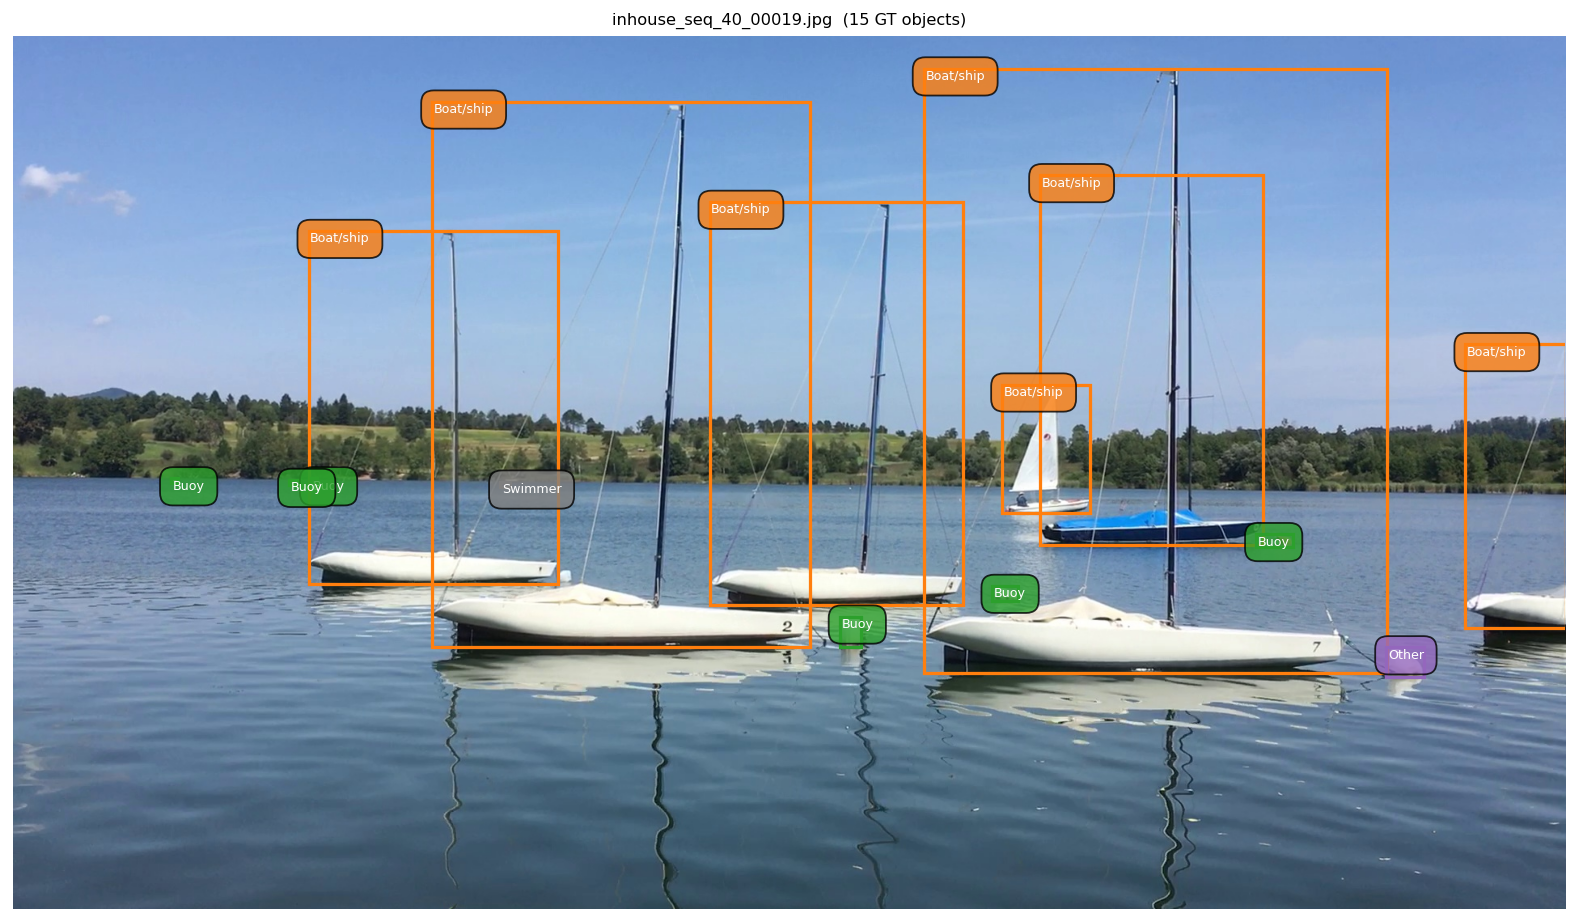
\includegraphics[width=\linewidth]{inhouse_seq_40_frame1_inhouse_seq_40_00019_gt.png}
        \caption{Frame 1}
    \end{subfigure}
    \begin{subfigure}{0.32\textwidth}
        \centering
        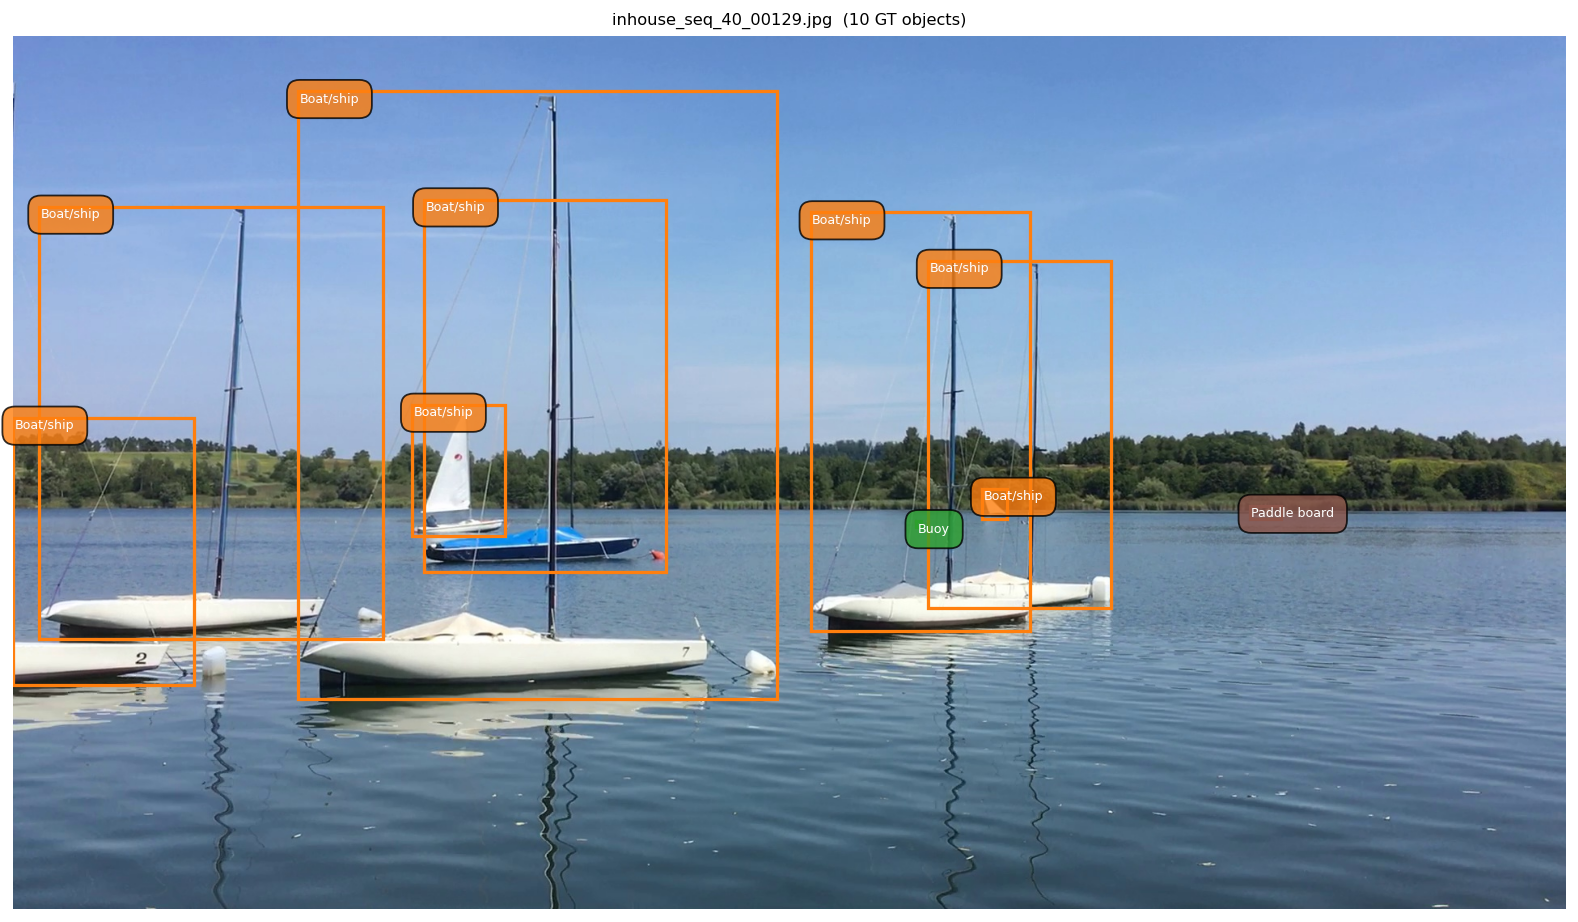
\includegraphics[width=\linewidth]{inhouse_seq_40_frame2_inhouse_seq_40_00129_gt.png}
        \caption{Frame 2}
    \end{subfigure}
    \begin{subfigure}{0.32\textwidth}
        \centering
        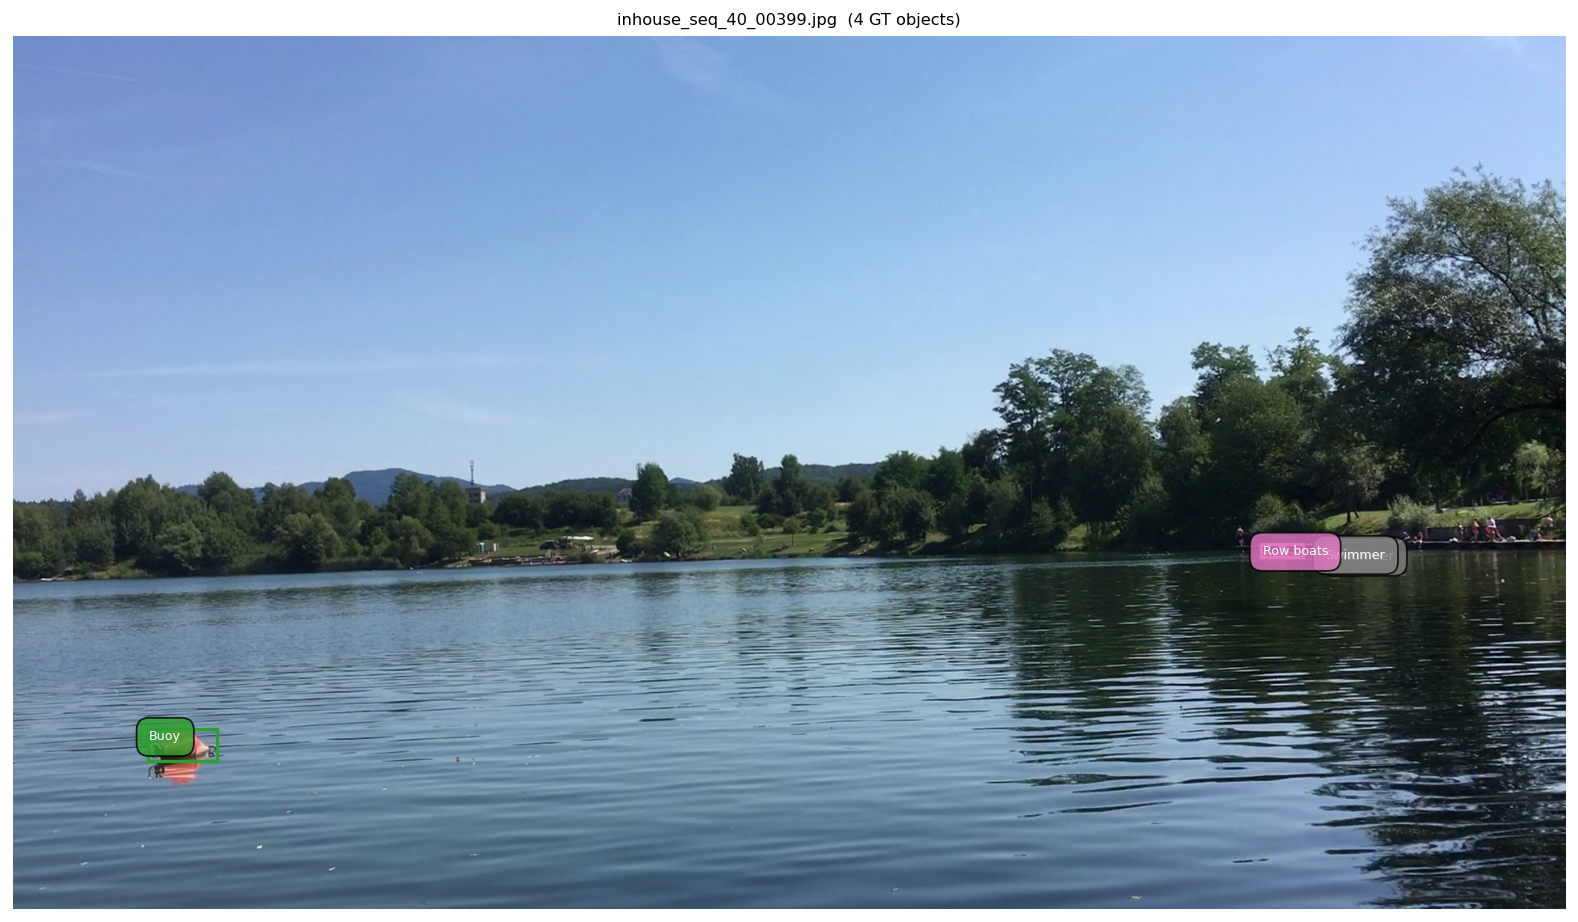
\includegraphics[width=\linewidth]{inhouse_seq_40_frame3_inhouse_seq_40_00399_gt.png}
        \caption{Frame 3}
    \end{subfigure}
    \caption{Three frames from one LaRS sequence (\texttt{inhouse\_seq\_40}) with
    ground-truth bounding boxes. The data comes in sequences, so each scene is
    captured over several frames.}
    \label{fig:data_samples}
\end{figure}

\subsection{Label Noise}
% TODO: Mention dataset is noisy; detailed handling in Methods.
Our detection boxes are not drawn by hand. They are the per-segment bounding boxes provided in the LaRS panoptic annotations. This works well for isolated objects, but the LaRS labels sometimes assign several distinct objects of the same class to a single segment, so its box spans all of them and the water between them. Some of these cases follow the dataset's convention of grouping nearby instances, but others are clear labeling errors it does not cover, with well-separated objects on opposite sides of the image sharing a single segment and box. This causes two linked errors: the large box is wrong, because it does not tightly enclose a single object, and the individual objects inside it appear to have no box of their own. Figure~\ref{fig:noise_examples} shows such a case. Because this noise can mislead both training and evaluation, we apply a model-assisted cross-validation relabeling step to clean the annotations; it is described in detail in Section~\ref{sec:relabel}.

\begin{figure}[H]
    \centering
    \begin{subfigure}{\textwidth}
        \centering
        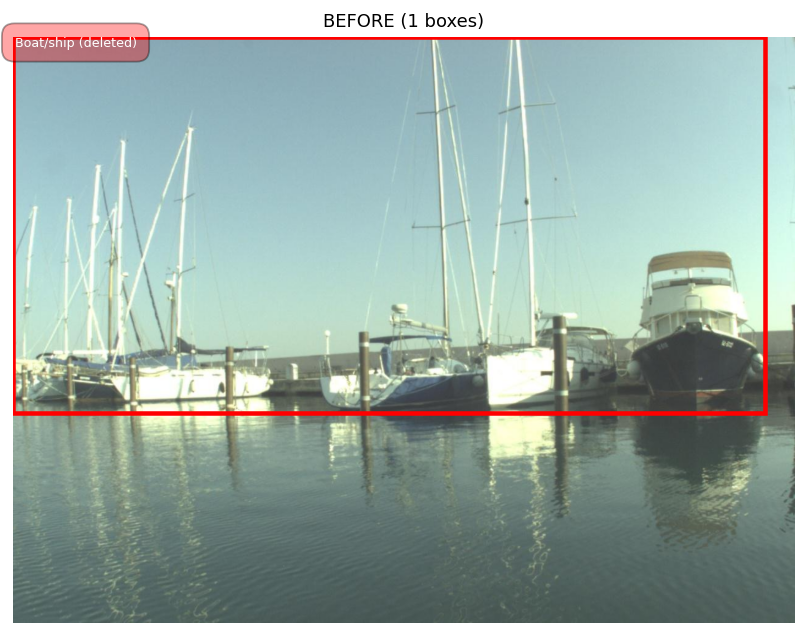
\includegraphics[width=0.7\linewidth]{relabel_before_mastr_0131_00009.png}
    \end{subfigure}

    \vspace{0.6em}

    \begin{subfigure}{\textwidth}
        \centering
        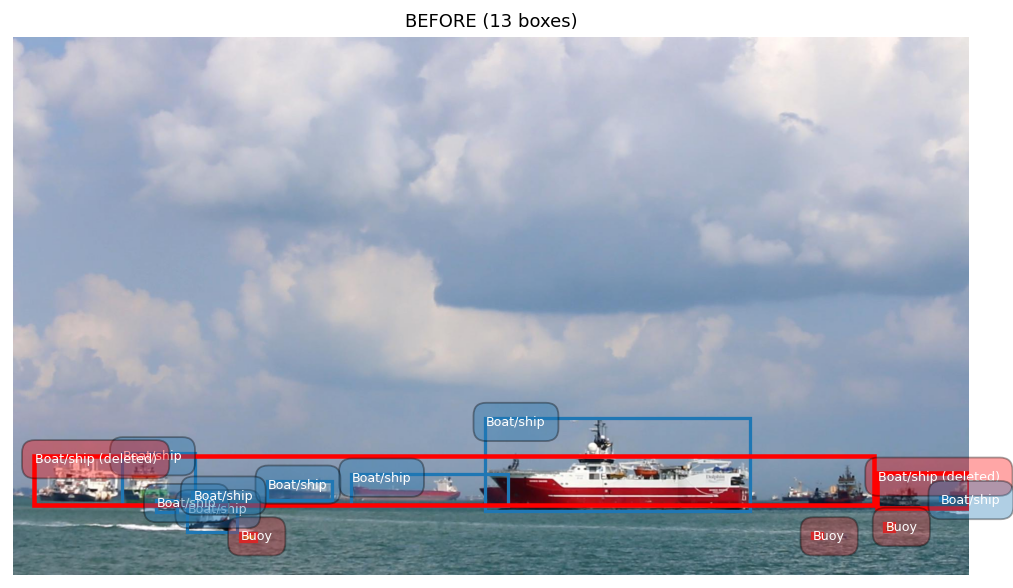
\includegraphics[width=0.7\linewidth]{relabel_before_smd_seq02_00172.png}
    \end{subfigure}
    \caption{Two examples of label noise in the LaRS detection annotations. A single oversized box covers several objects, and the individual objects inside it have no box of their own. The correction of this noise is shown later in Figure~\ref{fig:relabel_examples}.}
    \label{fig:noise_examples}
\end{figure}

\section{Methods}

\subsection{Preprocessing Pipeline}

\subsubsection{Scene-Level Data Split}
\label{sec:scene_split}
% TODO: Stratified scene-level split and leakage prevention.
We build our detection splits from the original LaRS train and validation data,
because these are the only splits with instance masks. From each panoptic mask we
keep the bounding box and class of every thing instance and drop the stuff
classes, giving a COCO-style detection dataset.

The original train split is divided into our train (80\%) and test (20\%) sets.
The split is done at the scene level: a scene is the source video, recovered by
removing the frame number from the file name (for example
\texttt{orca\_usv\_inland\_N03\_5\_00017.jpg} belongs to scene
\texttt{orca\_usv\_inland\_N03\_5}). All frames of a scene go to the same set, so
no near-duplicate frames leak between train and test.

To keep both sets representative, the split is stratified by scene attributes.
For each scene we take the dominant value of the four image-level labels
(\texttt{scene\_type}, \texttt{lighting}, \texttt{reflections}, \texttt{waves})
and combine them into one stratification key. Keys that occur for only a single
scene are merged into a shared ``rare'' bucket so the stratified split stays
valid. We use scikit-learn's stratified \texttt{train\_test\_split}. The original validation split is reused
unchanged, and the original test split is copied to an unused split with its
image-level labels only.

\subsubsection{Annotation Quality Issues}
% TODO: Mislabelled categories, noisy boxes, missing labels, ghost boxes, merged boxes.
As noted in the data description, the noise in our detection labels originates in the LaRS annotations themselves. A single panoptic segment, along with the bounding box LaRS provides for it, sometimes covers several distinct objects of the same class, giving one oversized box while those objects have no individual box of their own. The two errors therefore appear together: a wrong, too-large box on one side, and missing per-object boxes on the other. They are most harmful in dense scenes and for the small and rare classes, which already have few examples.

\subsubsection{Cross-Validation Relabeling}
\label{sec:relabel}
% TODO: RF-DETR fold model, held-out predictions, cleaning rules, provenance.
To reduce label noise without hand-checking every image, we use a model-assisted
cross-validation relabeling step. We pool all labelled images (train, validation,
and test) and split them into four scene-level folds, so that no scene appears in
more than one fold. For each fold $k$ we train an RF-DETR model on the other three
folds and run it on fold $k$. Because every image is only ever cleaned by a model
that did not see it during training, the predictions are unbiased held-out
predictions.

The model predictions, each with a confidence score, are compared against the
existing boxes to repair the grouped-segment errors. An existing box that does
not tightly match a single confident prediction, but instead overlaps several of
them, is treated as a wrong grouped box and deleted. A confident prediction that
matches no existing box is treated as a missing object and added as a new box.
The step removes the few oversized boxes that cover several objects and
regenerates the many per-object boxes that were missing inside them. Matching
uses an IoU threshold of 0.5, and confidence thresholds control when a box is
deleted or added so that only reliable predictions are kept. Every change is
written to a \texttt{provenance.json} file so the cleaning is fully traceable and
reversible.

Across the whole dataset this step changed 569 images: it removed 356 boxes and
added 677 boxes. For our train split, for example, the box count grows from 7{,}761
before cleaning to 8{,}025 after (522 added, 258 removed). The relabeled
annotations keep the original split membership and become the active labels used
for training and evaluation, while the pre-cleaning labels are kept alongside
them so the change is reversible.

\begin{figure}[H]
    \centering
    \begin{subfigure}{0.48\textwidth}
        \centering
        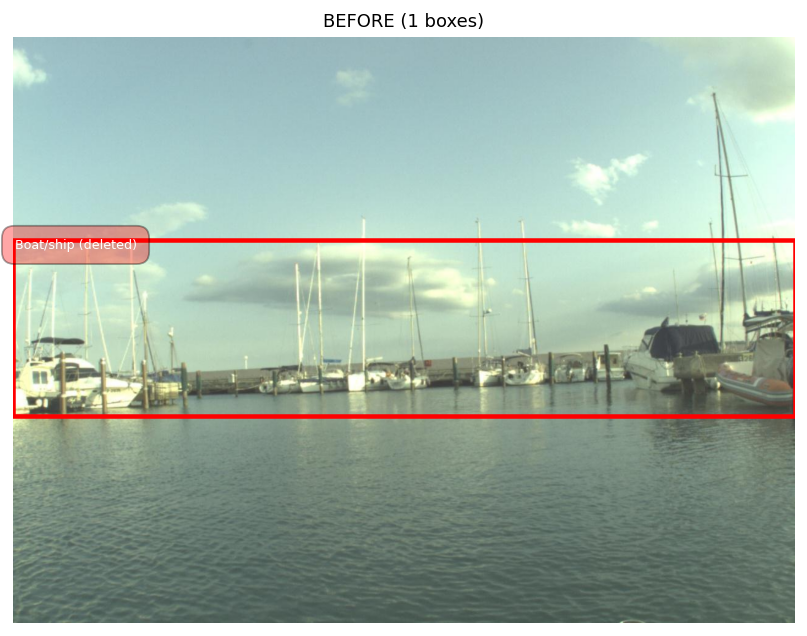
\includegraphics[width=\linewidth]{relabel_before_mastr_0687_00009.png}
        \caption{Before}
    \end{subfigure}\hfill
    \begin{subfigure}{0.48\textwidth}
        \centering
        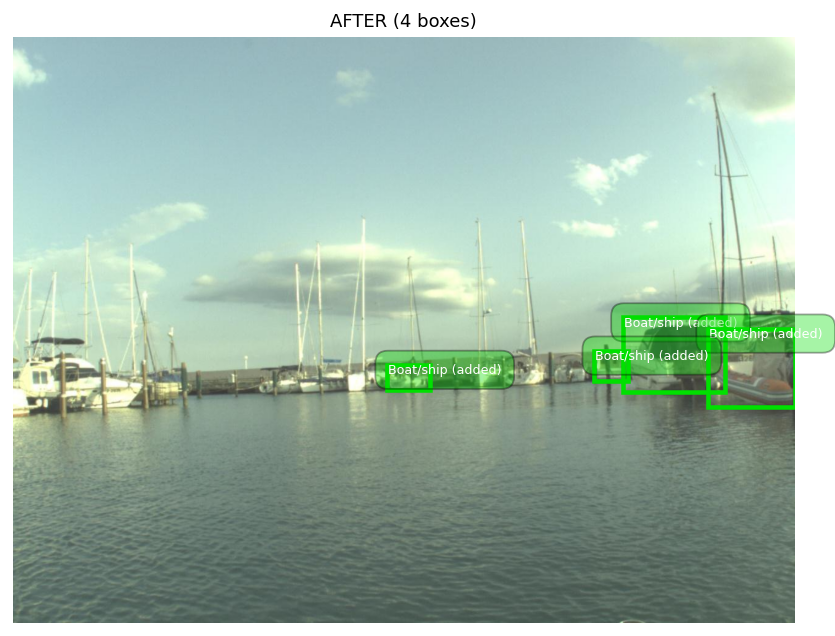
\includegraphics[width=\linewidth]{relabel_after_mastr_0687_00009.png}
        \caption{After}
    \end{subfigure}

    \vspace{0.6em}

    \begin{subfigure}{0.48\textwidth}
        \centering
        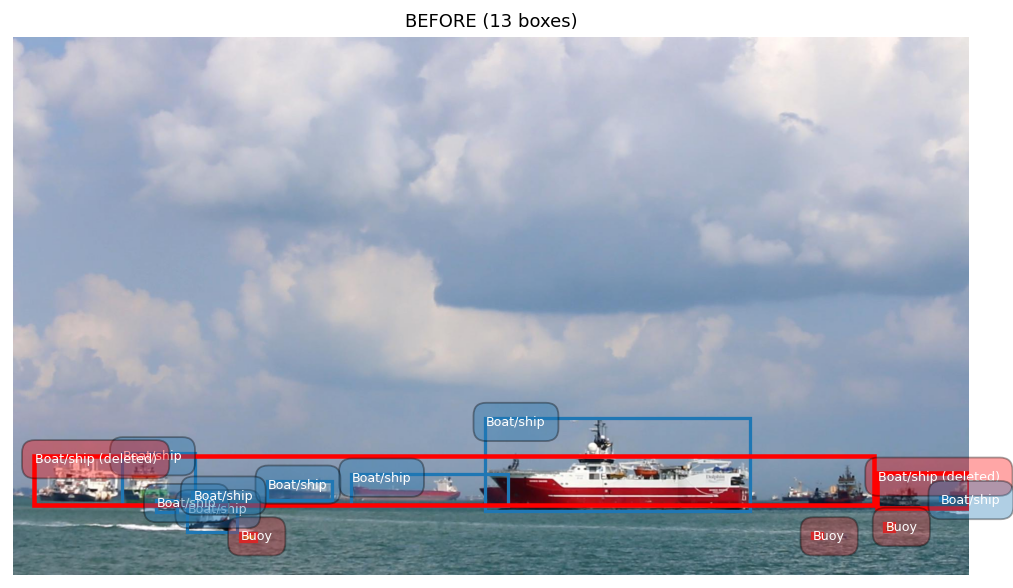
\includegraphics[width=\linewidth]{relabel_before_smd_seq02_00172.png}
        \caption{Before}
    \end{subfigure}\hfill
    \begin{subfigure}{0.48\textwidth}
        \centering
        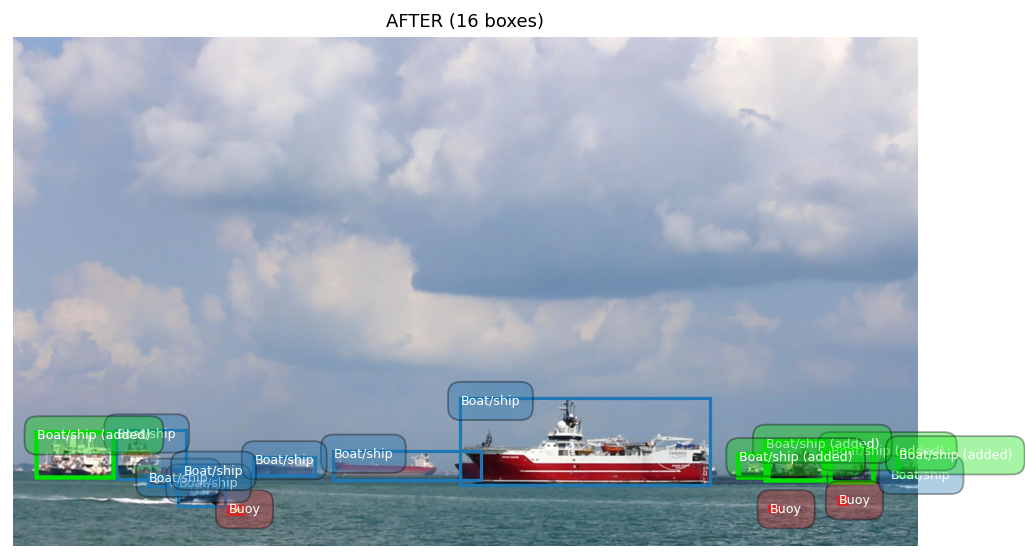
\includegraphics[width=\linewidth]{relabel_after_smd_seq02_00172.png}
        \caption{After}
    \end{subfigure}
    \caption{More examples of annotations before and after the cross-validation
    relabeling step: oversized boxes covering several objects are removed and a
    separate box is regenerated for each individual object.}
    \label{fig:relabel_examples}
\end{figure}

\subsubsection{Data Augmentation Strategy}
We treat data augmentation as part of the training configuration, not as a fixed
preprocessing step. No augmentation is permanently written into the stored
dataset: the canonical labels stay clean, and augmentation is only applied at
training time and can be undone.

The mechanism differs per model. For Faster R-CNN we apply online augmentation
with the Albumentations library, drawing from a small set of maritime-aware
policies (for example colour jitter, simulated fog and rain, or sensor noise).
For RF-DETR we use the same policies but as offline augmentation: a chosen number
of augmented copies of each image is written before training and removed again
afterwards, which is helpful for the rare classes on this small dataset. YOLOv8
uses its own built-in augmentations (such as colour jitter, flipping, scaling,
and mosaic).

Crucially, we do not fix the augmentation by hand. The augmentation policy and
its strength (and, for RF-DETR, the number of copies) are treated as tunable
hyperparameters and chosen by the Optuna search together with the other settings.
The exact augmentation search space for each model is given in
Section~\ref{sec:hpo}.

\subsection{Model Architectures}

\subsubsection{YOLOv8}
% TODO: One-stage detector, speed motivation, selected variants.
YOLOv8 is our one-stage CNN-based object detector. Unlike two-stage detectors
such as Faster R-CNN, it predicts object classes and bounding boxes directly in
one forward pass. This design reduces inference time and makes YOLOv8 suitable
for real-time applications such as autonomous maritime navigation.

The architecture consists of three main parts: a backbone, a neck, and a
detection head. The backbone extracts visual features from the input image using
convolutional layers and C2f blocks. Early layers mainly learn simple visual
patterns such as edges and textures, while deeper layers learn more abstract
features related to object shapes and object parts.

The neck combines feature maps from different spatial resolutions. It uses
upsampling and concatenation to transfer information between deeper and
shallower feature maps. This multi-scale feature fusion is important for the
LaRS dataset because maritime obstacles appear at very different sizes. A nearby
ship may occupy a large part of the image, while a distant buoy, swimmer, or
animal may cover only a small number of pixels.

The detection head uses the fused feature maps to predict object classes and
bounding-box coordinates at several scales. YOLOv8 uses an anchor-free detection
approach, so it predicts object locations directly instead of comparing them
with predefined anchor boxes. It also uses separate branches for classification
and bounding-box regression. This allows the two tasks to learn more specialised
features.

We evaluated the nano, small, and medium YOLOv8 variants during the
hyperparameter search. The final selected model was YOLOv8m, trained for
100 epochs with an input resolution of 1024 pixels and a batch size of 4.
The medium model provides a balance between representational capacity and
computational cost. The higher input resolution helps preserve more visual
detail, which is useful for small maritime objects. Its main advantage is fast
inference, while its main limitation in this project is the detection of very
small and visually ambiguous maritime objects.

\subsubsection{Faster R-CNN}
% TODO: Two-stage detector, ResNet-FPN backbone, region proposal network.
Faster R-CNN~\cite{fasterrcnn2015} is our two-stage baseline. Where YOLO is built
for speed, Faster R-CNN is built for accuracy: it first proposes regions that may
contain an object, and then classifies and refines each region. This split makes
it slower but usually more precise, which is why we use it as a strong reference
point.

\paragraph{Backbone.}
The image first goes through a ResNet-50 backbone with a Feature Pyramid Network
(FPN)~\cite{lin2017feature}. The FPN produces feature maps at several scales and
combines coarse, high-level features with fine, low-level detail. This helps with
a key problem in our data: many maritime obstacles (distant buoys, swimmers,
animals) are very small and easy to miss on a single-scale feature map.

\paragraph{Region proposal network.}
The first stage is the Region Proposal Network (RPN). It slides over the feature
maps and, at each location, compares a set of predefined anchor boxes of
different sizes and shapes against the objects. It outputs a set of candidate
regions that likely contain an object. The RPN is trained with a combined loss
that does two things at once: it learns whether an anchor contains an object, and
it learns how to adjust the anchor box to fit the object better:

\begin{equation}
L(\{p_i\}, \{t_i\}) = \frac{1}{N_{\text{cls}}} \sum_{i} L_{\text{cls}}(p_i, p_i^*)
  + \lambda \frac{1}{N_{\text{reg}}} \sum_{i} p_i^* \, L_{\text{reg}}(t_i, t_i^*).
\end{equation}

Here $p_i$ is the predicted object probability for anchor $i$ and $p_i^*$ its
ground-truth label, while $t_i$ and $t_i^*$ are the predicted and true box
adjustments. The first term is the classification loss (object vs.\ background)
and the second is the box-regression loss, which is only active for anchors that
contain an object ($p_i^* = 1$). The weight $\lambda$ balances the two terms.

The default anchors are made for everyday photos, not for water scenes, so we
replace them with anchors fitted to our data. The procedure is described in the
anchor analysis (Section~\ref{sec:hpo}).

\paragraph{Second stage.}
Each proposed region is cropped from the feature maps with RoIAlign~\cite{he2017mask},
which samples the region at a fixed size while keeping the coordinates exact. The
cropped features then go to two small heads: one classifies the region into one
of our 8 maritime classes (or background), and the other refines the box
coordinates. We use the COCO-pretrained ResNet-50-FPN model and replace only the
final layers to match our 8 classes.



\subsubsection{RF-DETR}
% TODO: Transformer-based detection architecture and current role as accuracy model.
RF-DETR~\cite{rfdetr2025} is our transformer-based detector. It builds on the
DETR family of models, so we first explain DETR, then what RF-DETR changes, and
finally how the model we use was pretrained.

\paragraph{From DETR to RF-DETR.}
DETR~\cite{carion2020detr} treats object detection as a direct set-prediction
problem. A CNN backbone turns the image into features, a transformer
encoder-decoder processes them, and a fixed set of learned ``object queries''
each predict one box and class. The output boxes are matched to the ground-truth
boxes one-to-one during training (bipartite matching), so DETR needs no anchor
boxes and no non-maximum suppression (NMS). This makes the pipeline simple, but
the original DETR has two well-known downsides: it is slow to train (it needs
many epochs to converge) and it is weak on small objects, partly because its
attention looks at the whole feature map at once.

RF-DETR keeps the clean DETR idea (set prediction, no anchors, no NMS) but fixes
these downsides in two main ways. First, it replaces the plain CNN backbone with
a \emph{DINOv2}~\cite{oquab2023dinov2} vision transformer backbone. DINOv2 is
pretrained in a self-supervised way on a very large set of images, so it already
has strong, general visual features. This gives RF-DETR a good ability to adapt
to new domains, even with relatively little training data. Second, it uses
\emph{deformable attention}~\cite{zhu2021deformable} in the decoder. Instead of
attending to every position in the feature map, each query only samples a few
relevant points around a reference location. This is much cheaper, converges
faster, and works better on small objects. RF-DETR also uses a single-scale
feature map from the backbone and a shallow decoder, which keeps it fast enough
for real-time use. Taken together, these changes are what make a DETR-style model
practical for a real-time system: RF-DETR is one of the first detectors of this
type to reach real-time speed while staying highly accurate.

\paragraph{Attention mechanism.}
The core mechanism is attention. In plain attention, every query position is
compared against every key position, which is accurate but expensive and scales
badly with image size. Deformable attention changes this: for each query, the
model predicts a small number of sampling offsets and only attends to the
features at those few points. This focuses the model on the spatially relevant
parts of the scene (for example the object itself), lowers the compute cost, and
helps the model find small objects such as buoys or swimmers. The same
attention weights can later be visualized to see where the model looks when it
makes a detection (see Figure~\ref{fig:xai_rfdetr_attention}).

\paragraph{Strengths and weaknesses.}
The main strengths of RF-DETR are: high accuracy combined with real-time speed;
strong transfer to new domains thanks to the DINOv2 pretraining, which suits a
specialized dataset like LaRS; a simple pipeline with no anchors and no NMS, so
there are fewer hand-set parameters; and good handling of small objects through
deformable attention. The main weaknesses are: transformer detectors generally
need more data and compute to train well than CNN detectors; the number of object
queries is fixed, which can limit very crowded scenes; and the model and its
tooling are newer and less mature than long-established detectors.

\paragraph{Pretraining of our model.}
We use the \texttt{RFDETRBase} variant, which has a DINOv2-Small (ViT-S) backbone
and about 29 million parameters. Its pretraining has two stages that we do not
repeat ourselves. The backbone is pretrained by DINOv2 in a self-supervised way
on a large image collection, without any detection labels. On top of this, the
authors release an RF-DETR detection checkpoint that is pretrained on the
Microsoft COCO object detection dataset. We start from this COCO-pretrained
checkpoint and fine-tune it on our (relabeled) LaRS detection data, using the
hyperparameters found by our search (Section~\ref{sec:hpo}). This transfer
learning is the standard way to use RF-DETR and lets us reach good accuracy
without training a transformer from scratch.

\subsubsection{Architecture Comparison}
% TODO: Expected speed/accuracy tradeoffs and suitability for maritime scenes.

\begin{table}[H]
    \centering
    \caption{Model families and expected tradeoffs.}
    \label{tab:model_overview}
    \begin{tabular}{llll}
        \toprule
        Model & Architecture type & Expected strength & Expected limitation \\
        \midrule
        YOLOv8 & TODO & TODO & TODO \\
        Faster R-CNN & TODO & TODO & TODO \\
        RF-DETR & TODO & TODO & TODO \\
        \bottomrule
    \end{tabular}
\end{table}

\subsection{Training Setup}
% TODO: Environment, seed, hardware, checkpoints, metrics logging.
All models are trained in PyTorch on a single NVIDIA A40 GPU. We do not train
any model from scratch. Instead we use transfer learning: each model starts from
weights that were pretrained on the Microsoft COCO detection dataset, and we
fine-tune it on our LaRS detection splits. For Faster R-CNN this is a
ResNet-50-FPN backbone with COCO-pretrained detection heads, for YOLOv8 the
official COCO-pretrained weights, and for RF-DETR the COCO-pretrained checkpoint
on top of its DINOv2 backbone (its pretraining is described in the RF-DETR
architecture section above).

To keep results reproducible we fix the random seed to 4 in all training and
search scripts. During training we evaluate on the validation split after each
epoch and log the losses and validation metrics (mAP) to a CSV file. We use
early stopping, so training stops when the validation mAP no longer improves, and
we keep the checkpoint with the best validation mAP as the final model for each
run.

\subsection{Hyperparameter Search}
\label{sec:hpo}
% TODO: Optuna setup, search spaces, study storage, smoke tests.
Good hyperparameters matter a lot on a small, imbalanced dataset, so we tune each
model with an automatic search using the Optuna framework. The setup is the same
for all three models. Each search runs a number of trials (10 by default), and in
each trial Optuna picks a set of hyperparameters, we train the model for a fixed,
shorter budget of epochs with early stopping, and we report the best validation
mAP back to Optuna. Optuna uses a Bayesian sampler (TPE), so later trials focus
on the regions of the search space that worked best. The studies are stored in an
SQLite database so a search can be paused and resumed, and we again fix the seed
to 4. The best trial per model gives the configuration we use for the final,
longer training run.

The tunable parameters differ per model, because each architecture exposes
different knobs.

\paragraph{YOLOv8.}
We search the model size (nano, small, or medium), the input image size
(640, 800, or 1024), the batch size, and the optimiser settings (initial and
final learning rate, momentum, weight decay, warm-up epochs) together with the
two loss weights (box and class). We also tune YOLOv8's built-in augmentations:
colour jitter (HSV), small rotations, translation, scaling, horizontal flip,
mosaic, and mixup.

\paragraph{RF-DETR.}
We search the learning rate and a separate, smaller learning rate for the
backbone (expressed as a ratio of the main rate), the weight decay, the gradient
clipping value, the input resolution (from 560 up to 784\,px), the batch size,
and the model variant (base or large). On top of this we tune an offline
augmentation policy and how many augmented copies of each image to add (0--3),
which helps the rare classes given the small training set.

\paragraph{Faster R-CNN.}
We search the learning rate and a smaller backbone learning rate, the weight
decay, the SGD momentum, the batch size, the learning-rate schedule (step size
and decay factor), and the augmentation policy. We also optionally use
repeat-factor oversampling to show rare classes more often. The anchor boxes are
\emph{not} searched here; they are set in advance by the anchor analysis
described next.

\subsubsection{Anchor Analysis (Faster R-CNN)}
Faster R-CNN relies on predefined anchor boxes, and its default anchors are
designed for everyday COCO objects, not for maritime scenes. We therefore analyse
the ground-truth boxes in the training split first. We look at the distribution
of box sizes and aspect ratios and compare them to the default anchors, which
shows that LaRS contains many very small objects and few of the wide or tall
shapes the defaults assume.

To pick better anchors, we run k-means clustering on the training-set box sizes,
using an IoU-based distance (the same idea as in YOLO) because box sizes scale
multiplicatively. We cluster into nine shapes and spread them over the five
feature-pyramid levels, from very small anchors for distant objects up to large
anchors for close-up ships. The resulting anchor sizes are
$\{8, 24\}$, $\{56, 96\}$, $\{112, 176\}$, $\{288, 320\}$, and $\{512, 624\}$
pixels across the five levels, with aspect ratios of $0.5$, $0.75$, and $1.25$.
These ratios are narrower than the defaults, which matches the box shapes we see
in the data. We use this fixed anchor configuration for all Faster R-CNN runs.

\subsection{Evaluation Methodology}
% TODO: mAP, precision, recall, F1, threshold sweeps, FPS, latency.
We evaluate every model on the same held-out test split along two axes:
detection accuracy and inference speed. All models read their classes from the
shared COCO annotation file, so the class indices are consistent across
architectures.

\subsubsection{Detection Accuracy}
% TODO: expand once final eval numbers are in.
For detection accuracy we report the standard COCO-style metrics: mean average
precision at IoU 0.50 (mAP@50), which is our main metric, and averaged over IoU 0.50--0.95 (mAP@50:95), as
well as precision, recall, and the F1 score. We also look at per-class
performance, since the strong class imbalance means the overall numbers are
dominated by the boat/ship class.

\subsubsection{Inference Speed Measurement}
% Source: 3_Model/inference_test.ipynb
Because the system is meant for a USV, speed matters as much as accuracy. We
measure inference speed under conditions that match real-time use: each model
runs on a single GPU and processes one image at a time (batch size~1). Every
model is loaded from its best checkpoint and receives images at its own training
resolution (RF-DETR at 784\,px, YOLOv8 at 800\,px, and Faster R-CNN at the native
image size), so each model is timed in the configuration it was trained for.

The timing follows a fixed warm-up and benchmark protocol. We first run 10
warm-up images that are not timed, to remove one-off start-up costs such as lazy
initialisation and memory allocation. We then time the next 50 images
individually. For each image we measure the wall-clock time around the full
prediction call with \texttt{time.perf\_counter()}; on the GPU we call
\texttt{torch.cuda.synchronize()} before recording the time, so that asynchronous
GPU work is fully included. The measured time is end-to-end per image and
therefore includes each model's own pre- and post-processing, not just the
network forward pass. The image set is sampled with a fixed random seed of 4 for
reproducibility.

From the per-image times we report the mean latency in milliseconds, its
standard deviation, and the resulting throughput in frames per second
(FPS~$=1000/\text{mean latency}$). For the qualitative comparison we additionally
run all models on a few sample images at a confidence threshold of 0.25 and plot
their predictions against the ground-truth boxes
(Figure~\ref{fig:inference_examples}).

\subsection{XAI Methodology}

\subsubsection{D-RISE}
% TODO: Model-agnostic object detection explanation approach.

D-RISE~\cite{petsiuk2021drise} is a model-agnostic explanation method for object detection. It can be
applied to YOLOv8, Faster R-CNN, and RF-DETR without requiring access to their
internal gradients or feature maps.

The method generates many random masks and applies them to the input image.
Each masked image is passed through the detector, and the resulting predictions
are compared with a selected target detection. The similarity score combines
bounding-box overlap, class agreement, and confidence.

The final saliency map is obtained by weighting the masks according to these
similarity scores. Regions that remain visible in masks with high scores receive
stronger saliency values.
As shown in Figure~\ref{fig:xai_drise}, warmer colours indicate image regions
that provide stronger support for the selected detection.
The same procedure is used for all three detectors, which allows a direct
qualitative comparison between the models.


\subsubsection{Grad-CAM++}
% TODO: Faster R-CNN explanation approach.

Grad-CAM++~\cite{chattopadhay2018grad} is a model-specific explanation method applied to 
our Faster R-CNN baseline. It uses a combination of internal feature maps and gradients 
to pinpoint which regions in the image are responsible for a specific object prediction. 
Compared to traditional Grad-CAM, the plus-plus variant provides better localization 
and is much more precise when handling images containing multiple objects of the same class.

We hook this visualization mechanism directly into layer 3 of the Feature Pyramid Network 
neck (\texttt{backbone.fpn.layer\_blocks[3]}). This layer handles multi-scale features right 
before they are processed into regional proposals, making it ideal for capturing structural 
shapes like vessel hulls and navigation markers.

To generate the map, the model selects the highest-confidence bounding box from a forward 
pass and calculates how much the target class score changes relative to the feature maps 
moving backward. The resulting positive weights are combined, upsampled to match the image size, 
and normalized. As shown in Figure~\ref{fig:xai_gradcam}, warmer colors pinpoint the exact 
structural geometry that convinced the model to make its final classification.

\subsubsection{EigenCAM}
% TODO: YOLO explanation approach.

EigenCAM is a gradient-free, model-specific explanation method applied to
YOLOv8. It uses internal feature maps to identify the dominant activation
pattern associated with a selected detection.

We use layer 15 of the YOLOv8 neck because its stride-8 feature map provides
relatively high spatial resolution, which is useful for the small and distant
objects in the LaRS dataset. The highest-confidence detection is selected, and
the corresponding region is cropped from the feature map.

Singular Value Decomposition is then used to extract the first principal
component of the cropped features. The resulting activation map is normalised,
resized, and overlaid on the input image. As shown in
Figure~\ref{fig:xai_eigencam}, warmer colours indicate stronger activations
within the selected bounding-box region.



\subsubsection{RF-DETR Attention Maps}
% TODO: Transformer attention visualization approach.
% Source: 5_XAI/XAI.ipynb (cross-attention map)
For RF-DETR we use a model-specific method that reads the model's own attention.
RF-DETR's decoder uses multi-scale deformable attention. Unlike plain DETR, it
does not build a dense attention map over the whole image. Instead, each object
query learns a small set of \emph{sampling locations} in the feature maps, and
each location gets an \emph{attention weight}. These points are where the query
actually looks.

To visualize this, we attach a hook to the last decoder layer and read out the
sampling locations and their attention weights for the query that produced the
target detection (the highest-confidence box). We then place each attention
weight at its sampling point on an empty, image-sized map, summing over the
attention heads and feature levels. The map is lightly blurred and normalised to
the range $[0, 1]$, and finally overlaid on the input image as a heatmap. Bright
areas show the points that most influenced the detection. As for the other
methods, we run this on the test split with a fixed seed of~4, using RF-DETR's
detection threshold of 0.4. The result is shown in
Figure~\ref{fig:xai_rfdetr_attention}.

\section{Results}

\subsection{Model Performance Overview}
% TODO: Main quantitative comparison table.
Table~\ref{tab:model_results} compares the best variant of each model family on
our test split, on both accuracy and speed.

\begin{table}[H]
    \centering
    \caption{Model comparison on the test split, using the best variant of each
    model family. Detection metrics are in percent; precision and recall are
    taken at each model's best-F1 confidence threshold. FPS is measured on a
    single GPU at batch size~1. Best value per column in bold.}
    \label{tab:model_results}
    \begin{tabular}{lrrrrr}
        \toprule
        Model & mAP@50:95 & mAP@50 & Precision & Recall & FPS \\
        \midrule
        YOLOv8       & 23.4 & 42.2 & 70.8 & 60.1 & \textbf{49.8} \\
        Faster R-CNN & 23.5 & 43.6 & 72.9 & 57.8 & 20.3 \\
        RF-DETR      & \textbf{34.1} & \textbf{58.6} & \textbf{81.2} & \textbf{67.7} & 27.2 \\
        \bottomrule
    \end{tabular}
\end{table}

RF-DETR is the clear winner on accuracy. It reaches 34.1 mAP@50:95 and 58.6
mAP@50, clearly ahead of Faster R-CNN (23.5 / 43.6) and YOLOv8 (23.4 / 42.2), and
it also has the best precision (81.2\%) and recall (67.7\%). The two CNN baselines
are close to each other in accuracy. On speed the order is reversed: YOLOv8 is
the fastest at 49.8 FPS, RF-DETR still runs in real time at 27.2 FPS, and Faster
R-CNN is the slowest at 20.3 FPS. So RF-DETR gives the best accuracy while staying
fast enough for real-time use, while YOLOv8 is the best choice when raw speed is
the priority.

\subsection{Confusion Matrices}

\begin{figure}[H]
    \centering
    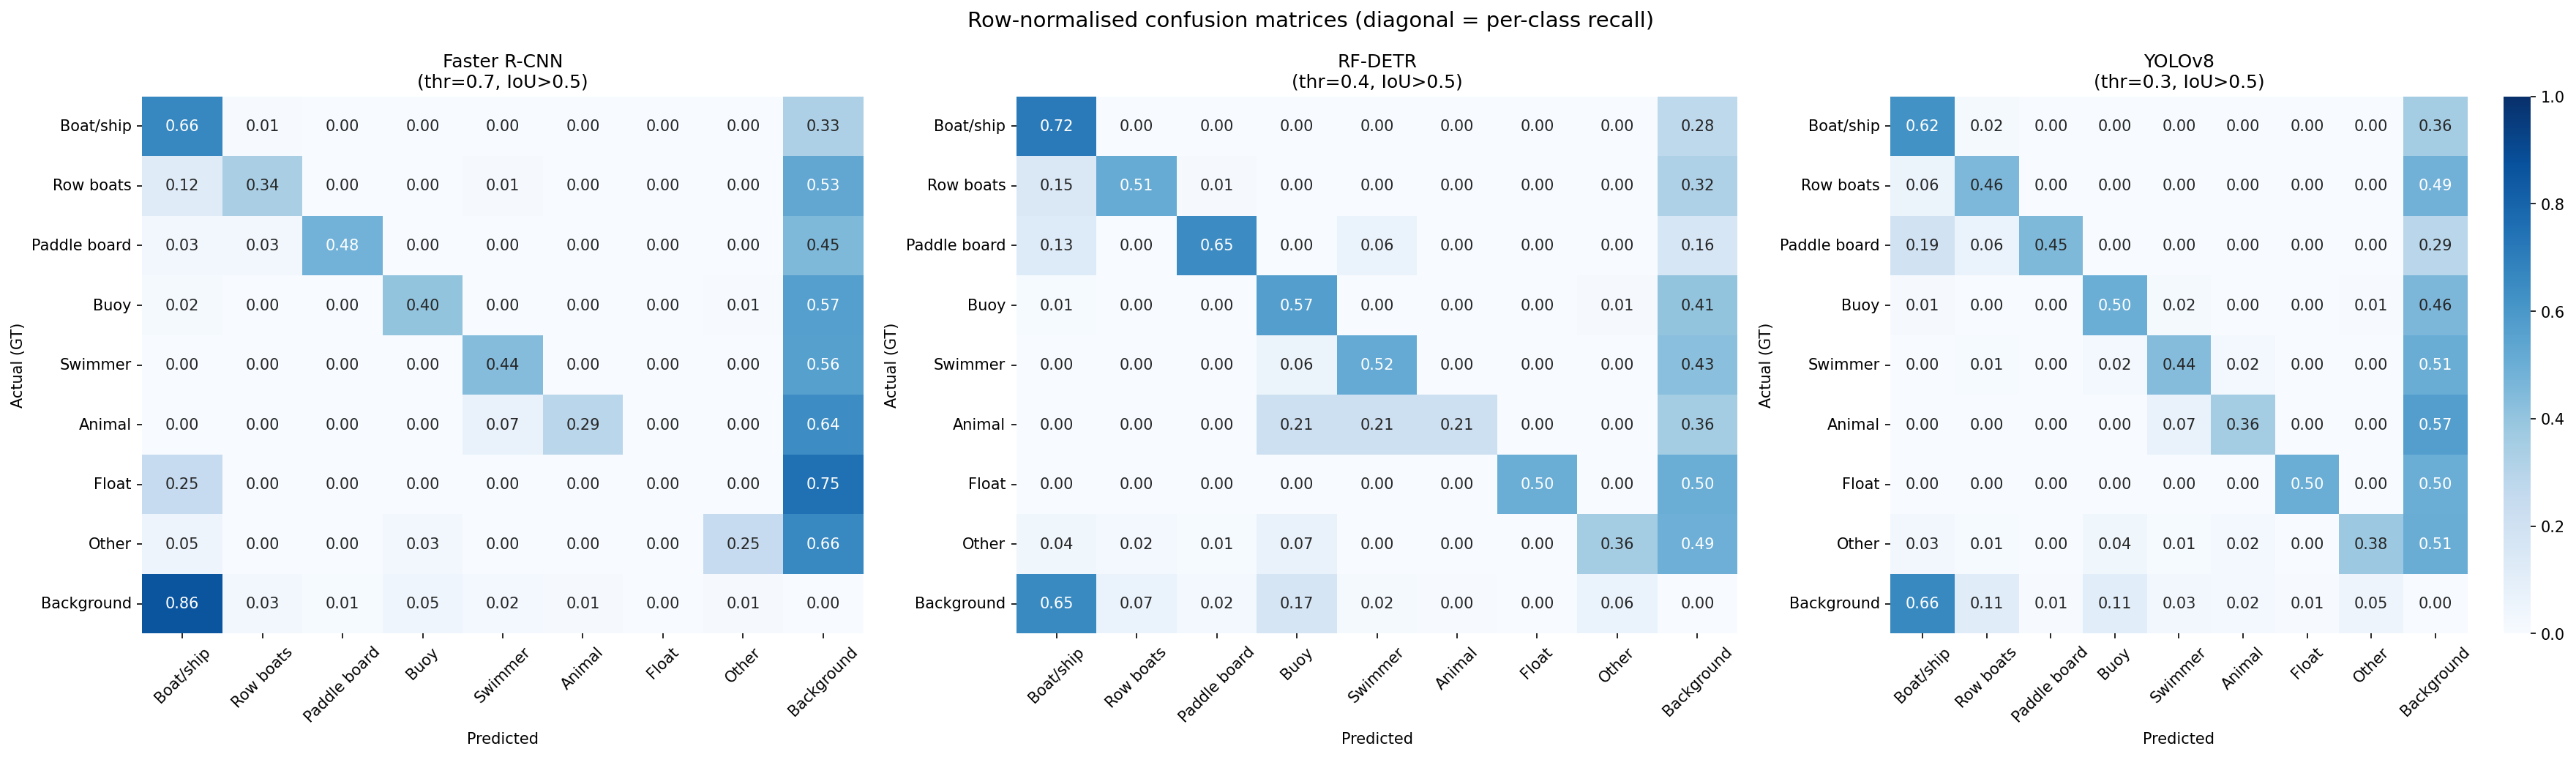
\includegraphics[width=\textwidth]{confusion_matrix_rownorm_all_models.png}
    \caption{Row-normalised confusion matrices for all evaluated models. Each row
    is normalised over the ground-truth class, so the diagonal shows per-class
    recall.}
    \label{fig:confusion_matrices}
\end{figure}

Two patterns stand out in Figure~\ref{fig:confusion_matrices}. First, RF-DETR has
the highest recall on almost every class (the strongest diagonal). Second, for all
three models the largest errors sit in the \emph{Background} column, which means
the main problem is missing objects, not confusing one class with another.
Genuine class confusion is small, and where it happens the rare classes (row
boats, paddle boards, floats) are mostly mistaken for the dominant boat/ship
class. The rare classes are hardest for everyone: Faster R-CNN never detects
floats, while RF-DETR and YOLOv8 reach about 50\% recall on them, and the animal
class stays weak across all models.

\subsection{Object Size Distribution And Error Analysis}
To understand \emph{where} the errors come from, we break the detections down by
object size. Figure~\ref{fig:size_distribution} shows, for each model and over the
bounding-box area, how many objects are correctly detected (true positives),
missed (false negatives), or wrongly predicted (false positives).

\begin{figure}[H]
    \centering
    \begin{subfigure}{\textwidth}
        \centering
        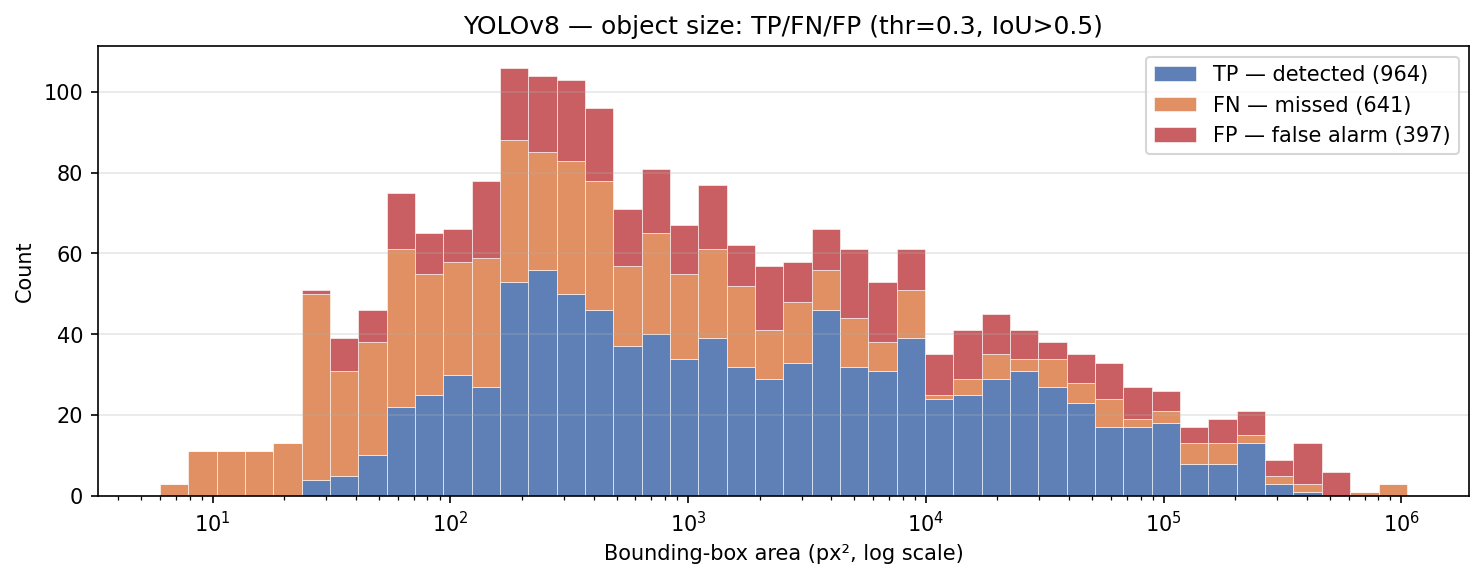
\includegraphics[width=0.8\linewidth]{size_distribution_yolo.png}
        \caption{YOLOv8}
    \end{subfigure}

    \begin{subfigure}{\textwidth}
        \centering
        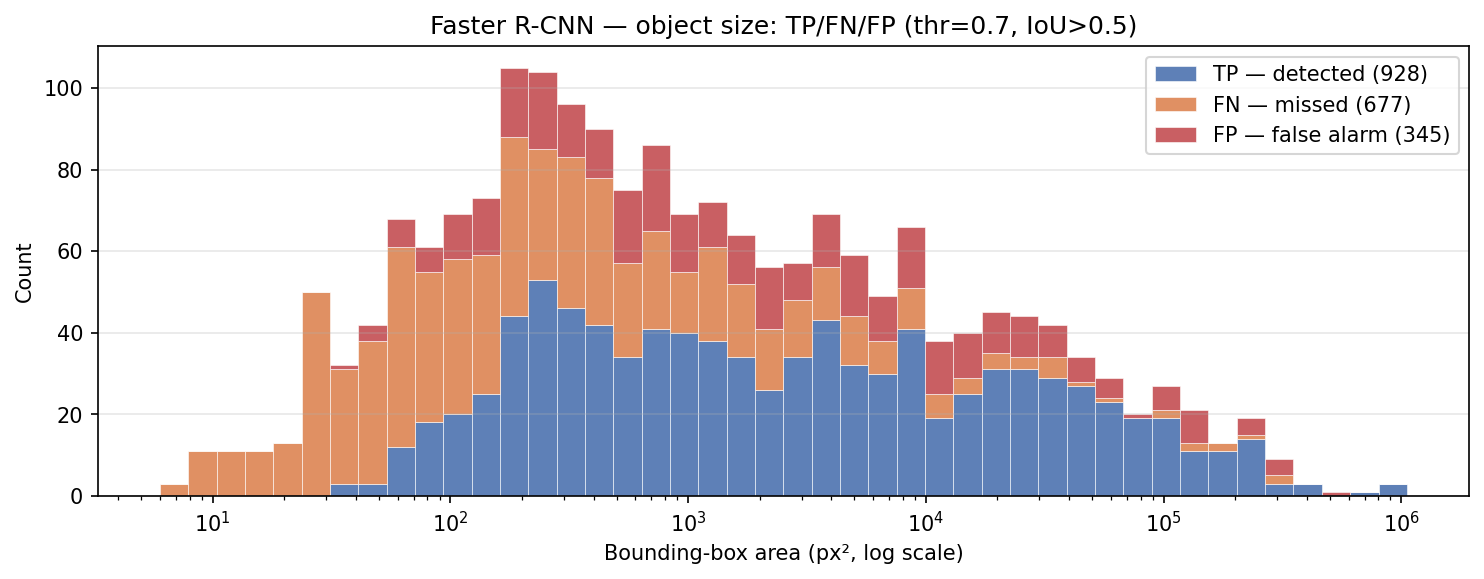
\includegraphics[width=0.8\linewidth]{size_distribution_fasterrcnn.png}
        \caption{Faster R-CNN}
    \end{subfigure}

    \begin{subfigure}{\textwidth}
        \centering
        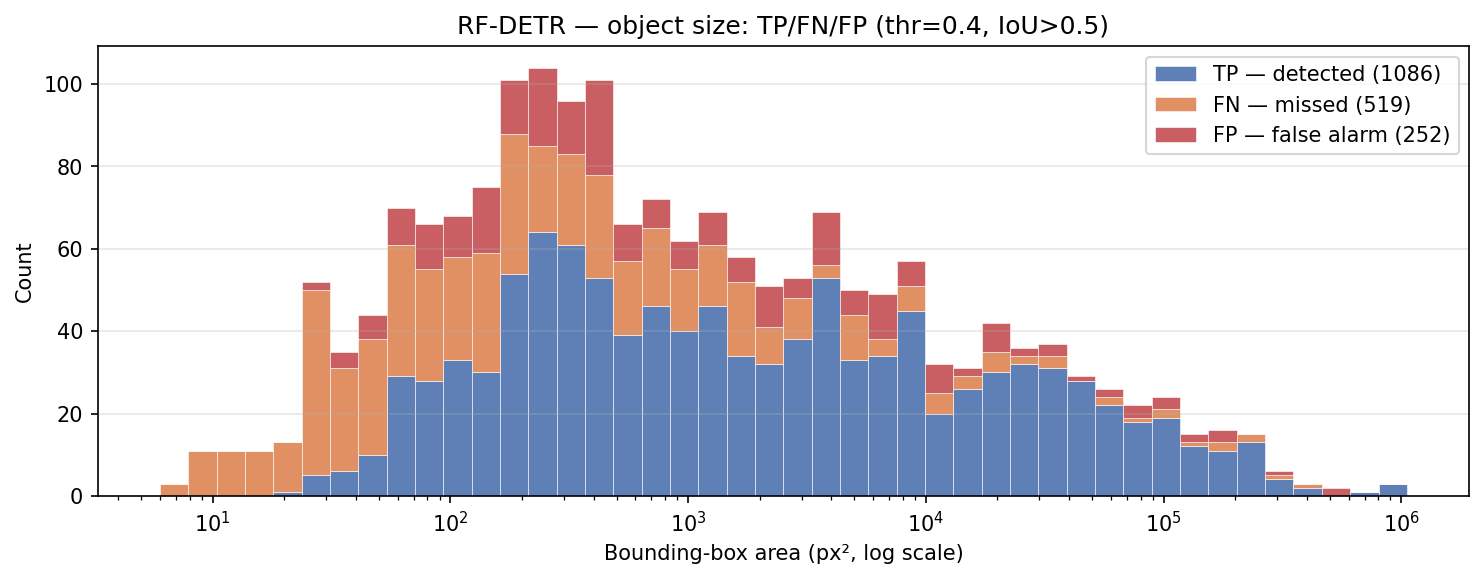
\includegraphics[width=0.8\linewidth]{size_distribution_rfdetr.png}
        \caption{RF-DETR}
    \end{subfigure}
    \caption{True positives, missed objects (false negatives) and false alarms
    (false positives) per model, as a function of bounding-box area (log scale).}
    \label{fig:size_distribution}
\end{figure}

The misses are concentrated on small objects on the left of each plot, while
larger objects are detected more reliably. The very smallest objects (a few hundred
square pixels and below) are missed by all three models. RF-DETR makes fewer
mistakes than the other two across the whole size range, with both fewer misses and
fewer false alarms, and recovers more of the small objects (1{,}087 true
positives vs.\ 964 for YOLOv8 and 928 for Faster R-CNN). Faster R-CNN misses the
most objects overall (677 false negatives), and YOLOv8 produces the most false
alarms (397 false positives).

\subsection{False Positive and False Negative Analysis}
To see \emph{what} the models get wrong, Figure~\ref{fig:fp_fn} shows example
crops of false positives and false negatives for each model. The missed objects
are small, distant obstacles and objects where the ground truth label also seems off. Some of these objects the model also correctly identifies as an object but predicts the wron labl. As we saw in the confusion matrix, the models sometimes don't classify small objects like bouyes and animals correctly but also mix up ships from row boats or paddle boat. This is consistent with the size
analysis above: small objects and water artefacts are the main sources of error.

\begin{figure}[H]
    \centering
    \begin{subfigure}{\textwidth}
        \centering
        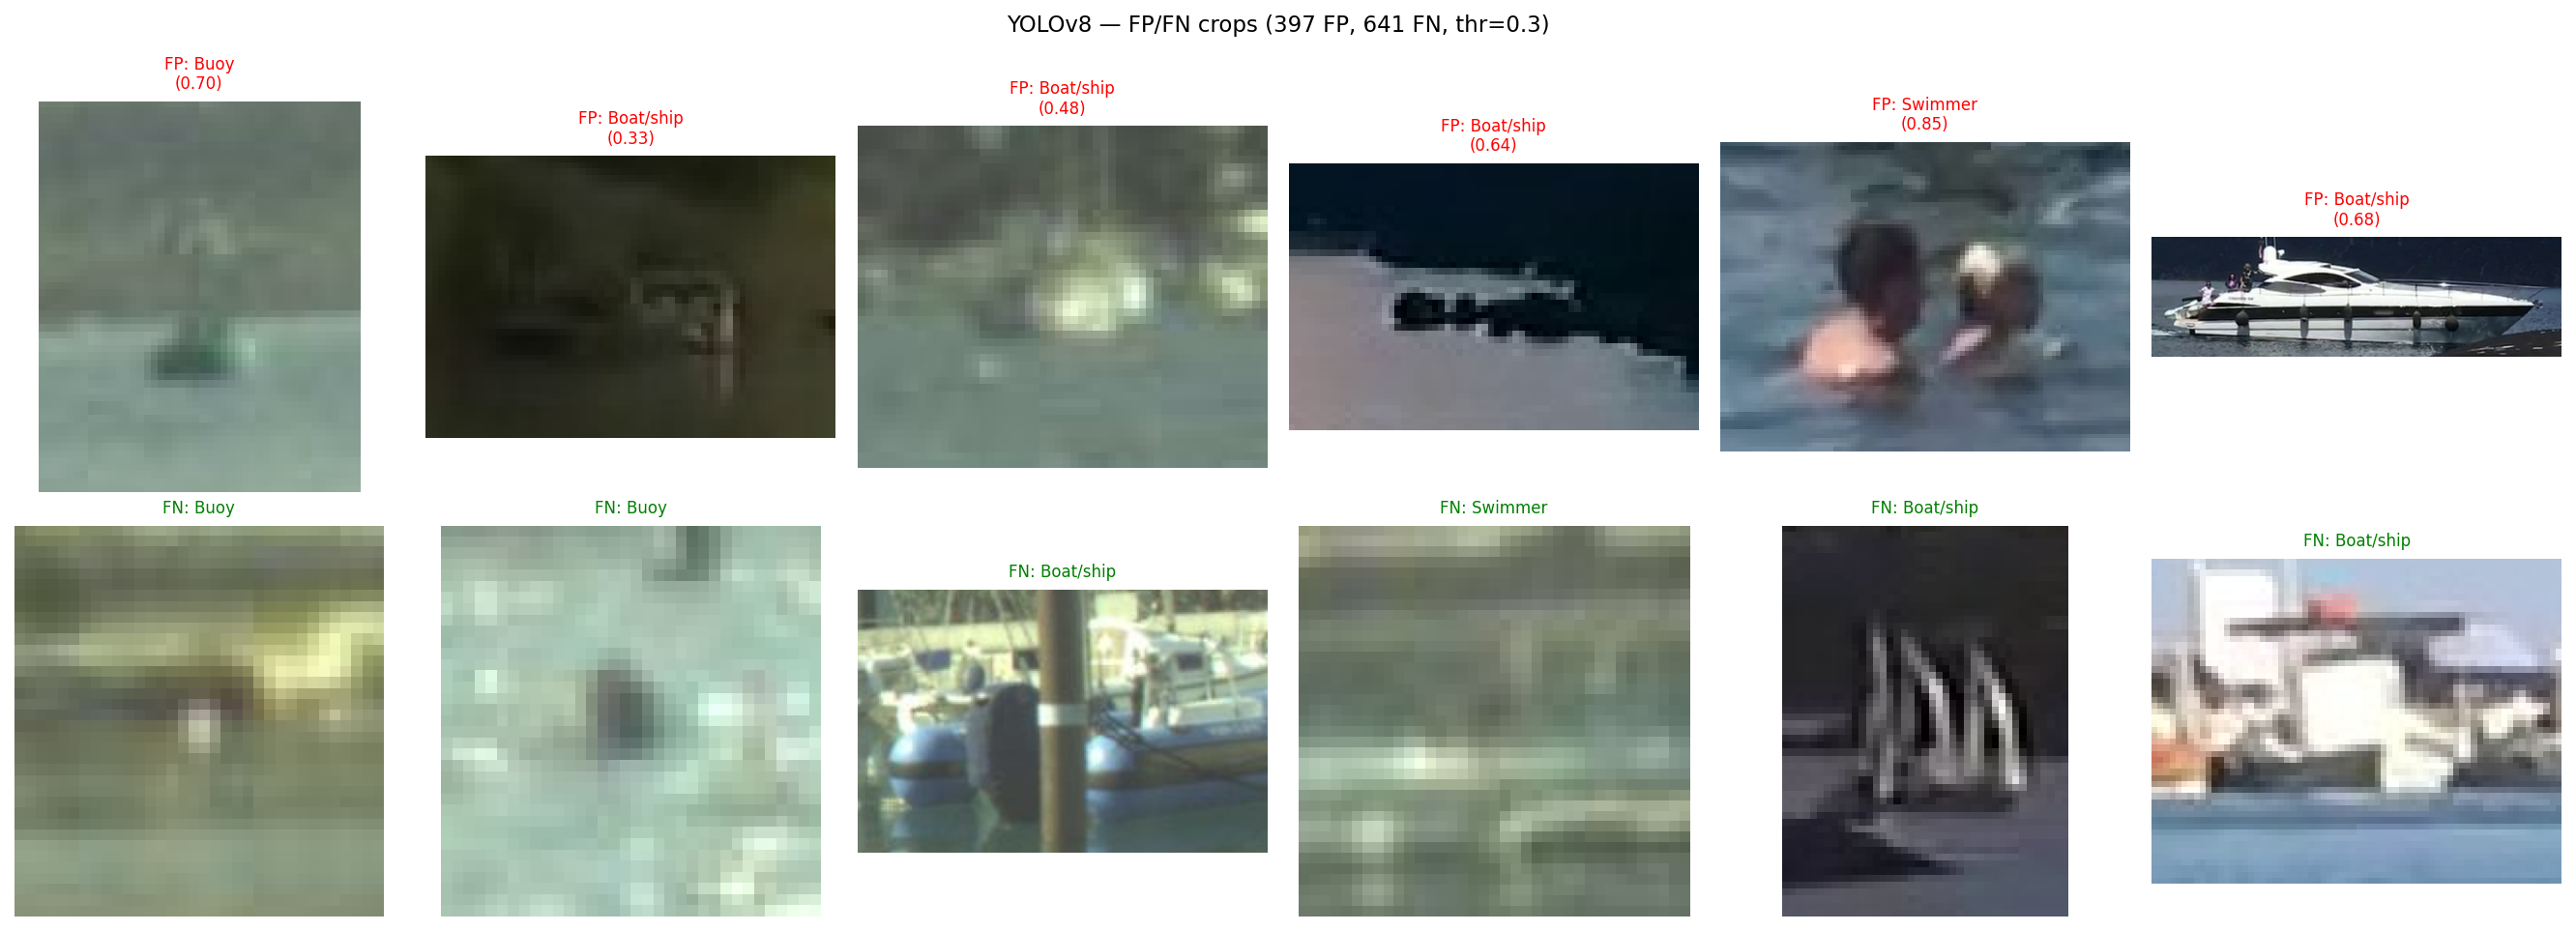
\includegraphics[width=0.85\linewidth]{fp_fn_crops_yolo.png}
        \caption{YOLOv8}
    \end{subfigure}

    \begin{subfigure}{\textwidth}
        \centering
        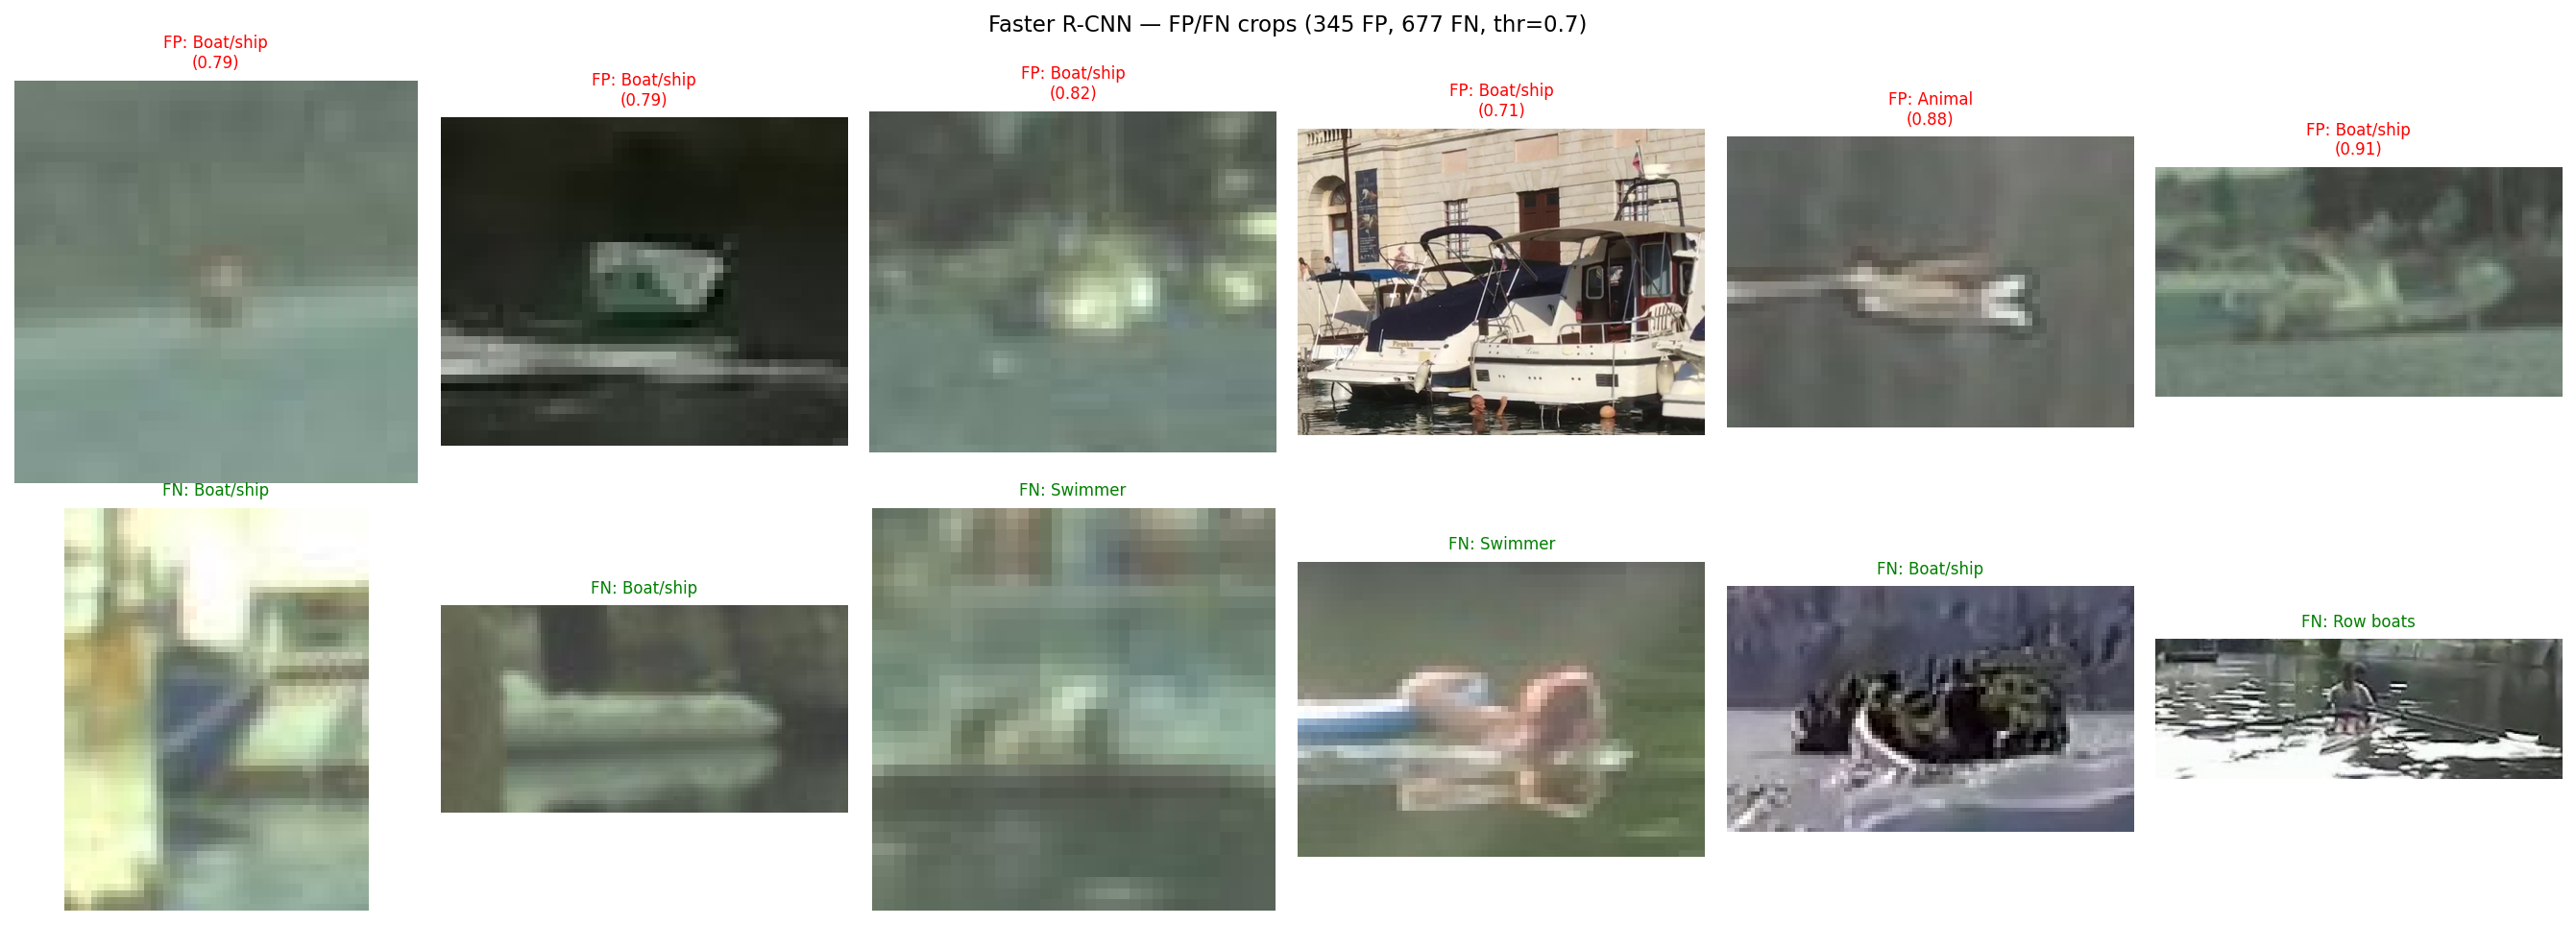
\includegraphics[width=0.85\linewidth]{fp_fn_crops_fasterrcnn.png}
        \caption{Faster R-CNN}
    \end{subfigure}

    \begin{subfigure}{\textwidth}
        \centering
        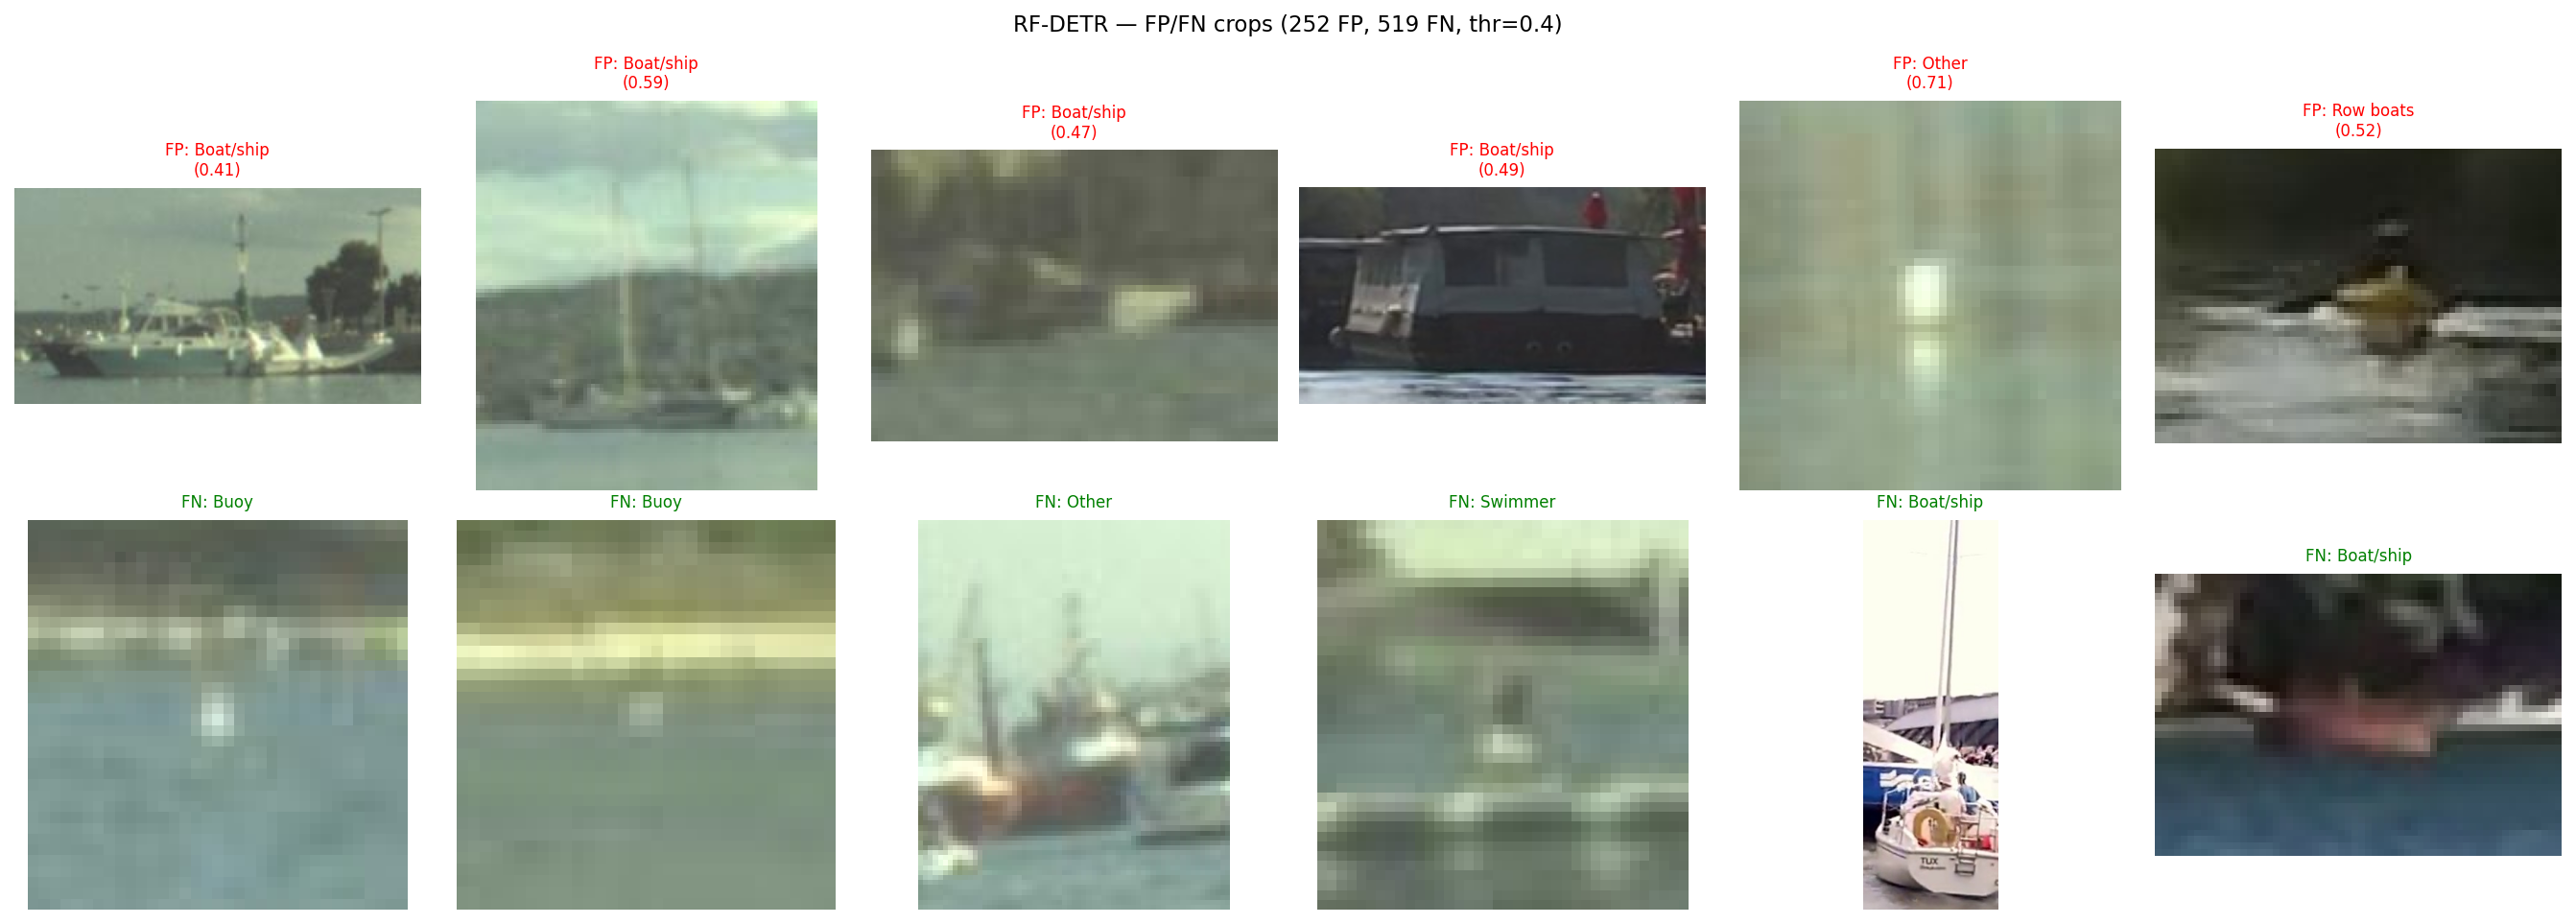
\includegraphics[width=0.85\linewidth]{fp_fn_crops_rfdetr.png}
        \caption{RF-DETR}
    \end{subfigure}
    \caption{Example false-positive and false-negative crops for each model.}
    \label{fig:fp_fn}
\end{figure}

\subsection{Inference Tests}
To see how the models behave on real footage, we ran them on frames from a
recorded video. Figure~\ref{fig:inference_examples} shows the detections of the
three models on the same example frame.

\begin{figure}[H]
    \centering
    \begin{subfigure}{\textwidth}
        \centering
        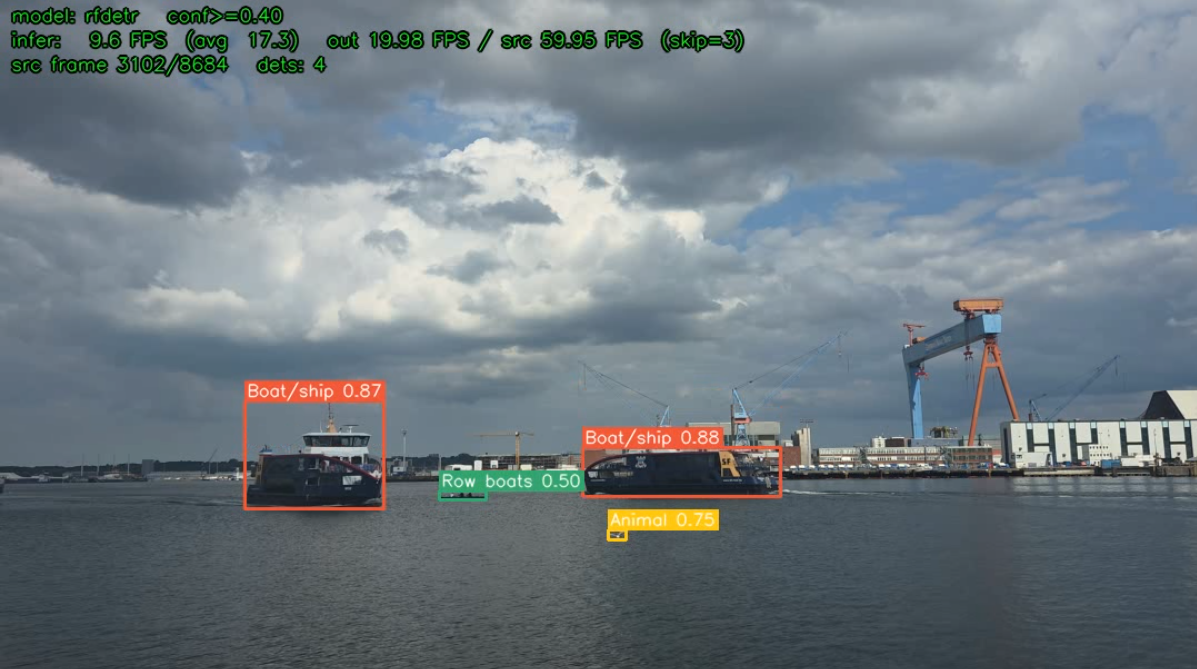
\includegraphics[width=0.6\linewidth]{rfdetr_qualitative_frame_50.png}
        \caption{RF-DETR}
    \end{subfigure}

    \begin{subfigure}{\textwidth}
        \centering
        
\includegraphics[width=0.6\linewidth]{images/yolo_qualitative_frame_50_2.png}
        \caption{YOLOv8}
    \end{subfigure}

    \begin{subfigure}{\textwidth}
        \centering
        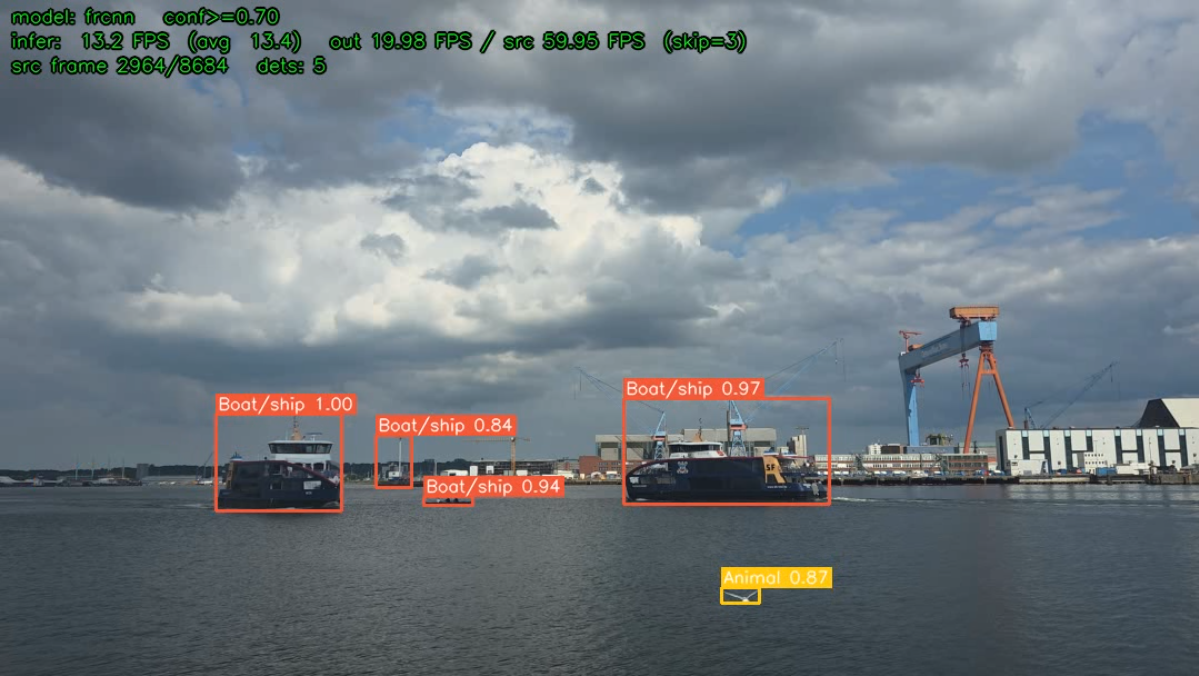
\includegraphics[width=0.6\linewidth]{frcnn_qualitative_frame.png}
        \caption{Faster R-CNN}
    \end{subfigure}
    \caption{Qualitative detection examples of the three models on the same video
    frame.}
    \label{fig:inference_examples}
\end{figure}

In the example frame, all models correctly detect the large ship in the middle,
although the box sometimes flickers when a model is unsure of its size. A row boat
in the middle is also found by all models, but Faster R-CNN and YOLOv8 tend to
label it as a boat/ship, while RF-DETR more often gives it the correct row-boat
class. When a bird flies into the scene, RF-DETR classifies it correctly as the
animal class more often than the others; YOLOv8 usually predicts the open-world
``other'' class, and Faster R-CNN is sometimes correct. Overall, RF-DETR looks the
most stable, while all three models work but produce noisy, flickering
predictions. This suggests that frame smoothing or other live-inference techniques
would be needed for more reliable results in practice.



\subsection{XAI Results}

\subsubsection{D-RISE Results}
D-RISE is model-agnostic, so we can apply it to all three detectors and compare
them directly.

\begin{figure}[H]
    \centering
    \begin{subfigure}{\textwidth}
        \centering
        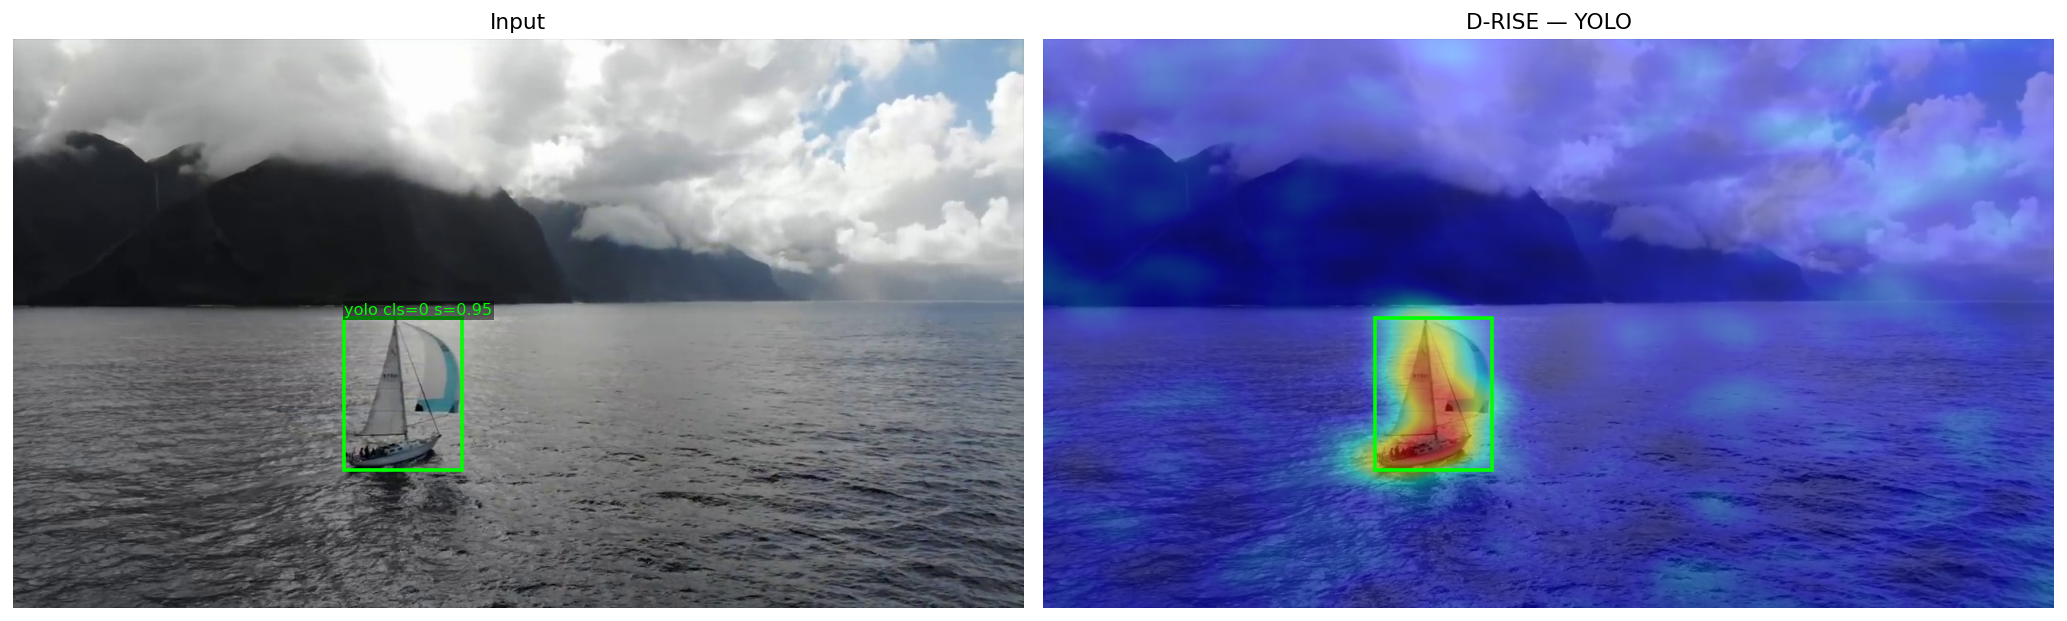
\includegraphics[width=0.85\linewidth]{xai_drise_yolo.png}
        \caption{YOLOv8}
    \end{subfigure}

    \begin{subfigure}{\textwidth}
        \centering
        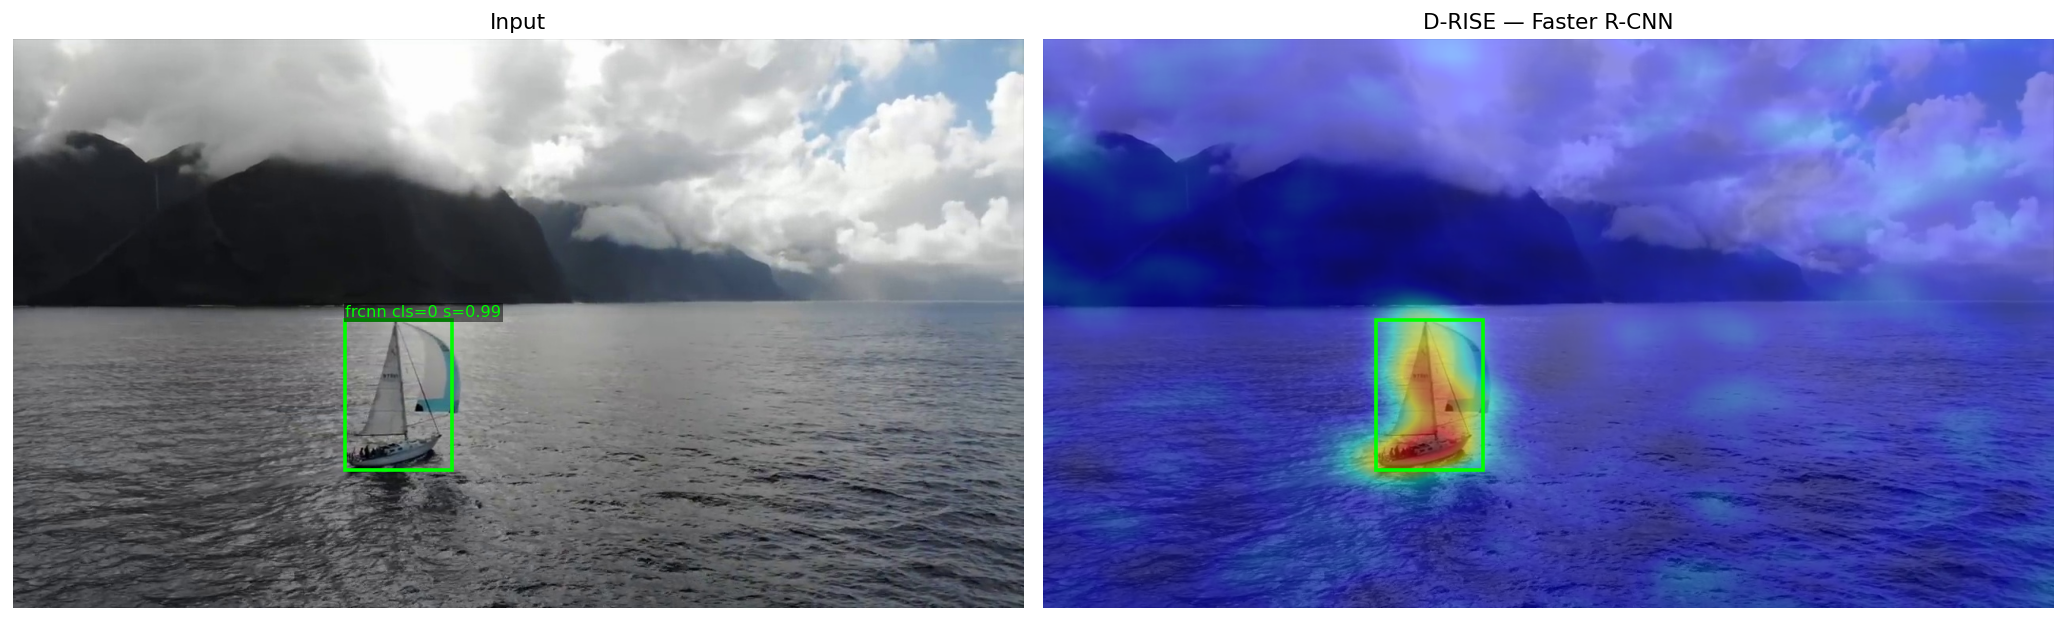
\includegraphics[width=0.85\linewidth]{xai_drise_fasterrcnn.png}
        \caption{Faster R-CNN}
    \end{subfigure}

    \begin{subfigure}{\textwidth}
        \centering
        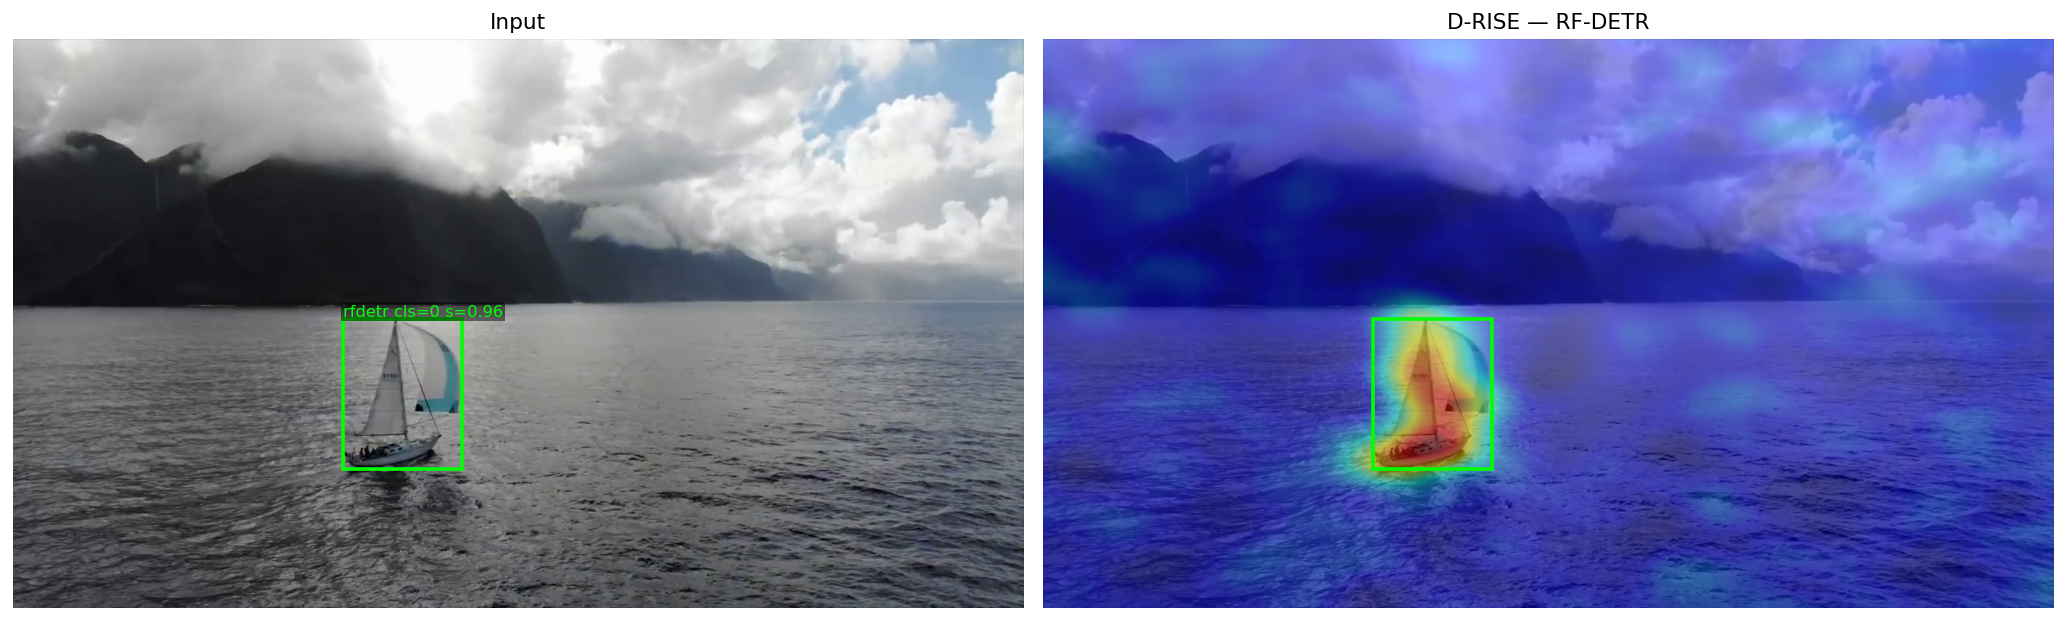
\includegraphics[width=0.85\linewidth]{xai_drise_rfdetr.png}
        \caption{RF-DETR}
    \end{subfigure}
    \caption{D-RISE saliency maps for the three detectors on the same scene.
    Brighter regions are the areas that most support the detection.}
    \label{fig:xai_drise}
\end{figure}

\subsubsection{Grad-CAM++ Results}

Figure~\ref{fig:xai_gradcam} shows the Grad-CAM++ activation map generated from the Feature Pyramid Network neck of our Faster R-CNN model. The map explains the features supporting the highest-confidence boat detection (\texttt{box 0}) with a confidence score of 88\% ($s = 0.88$). 

The warmest red and yellow regions are concentrated directly on the vessel's hull and main physical structure. Conversely, the surrounding open water, wave profiles, and background ripples are suppressed in dark blue, low-activation tones. This target-centric focus confirms that the model relies on the actual structural shape of the object rather than background water textures or environmental noise.

\begin{figure}[H]
    \centering
    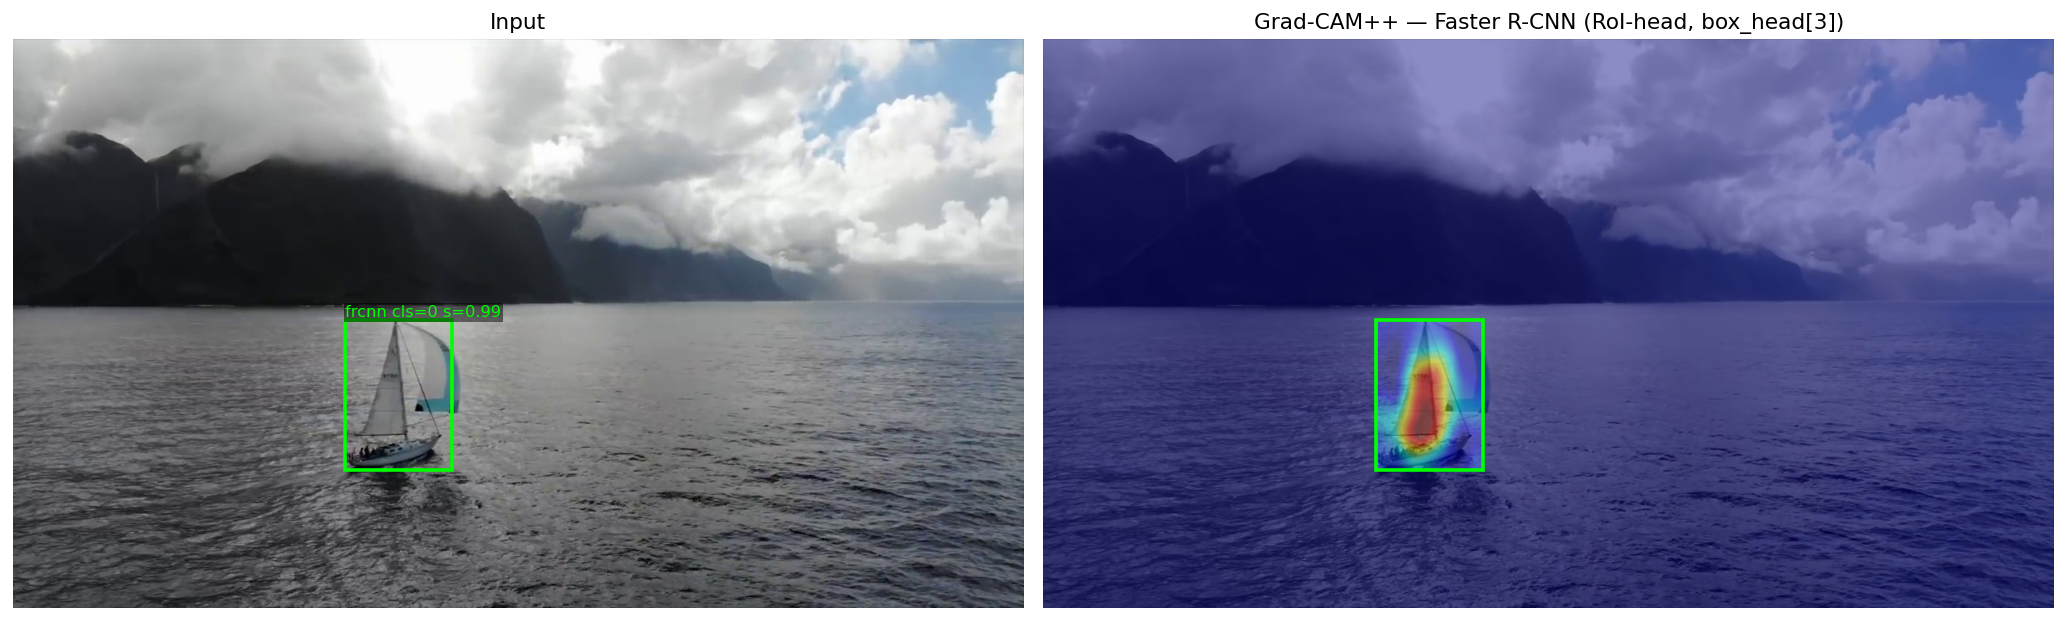
\includegraphics[width=0.85\textwidth]{xai_gradcampp_fasterrcnn.png}
    \caption{Grad-CAM++ explanation for Faster R-CNN.}
    \label{fig:xai_gradcam}
\end{figure}

\subsubsection{EigenCAM Results}
Figure 11 shows the distribution of EigenCAM activations within the selected YOLOv8 bounding box. The strongest activations appear around the hull and lower sail region, while the upper part of the sail has weaker activations.


\begin{figure}[H]
    \centering
    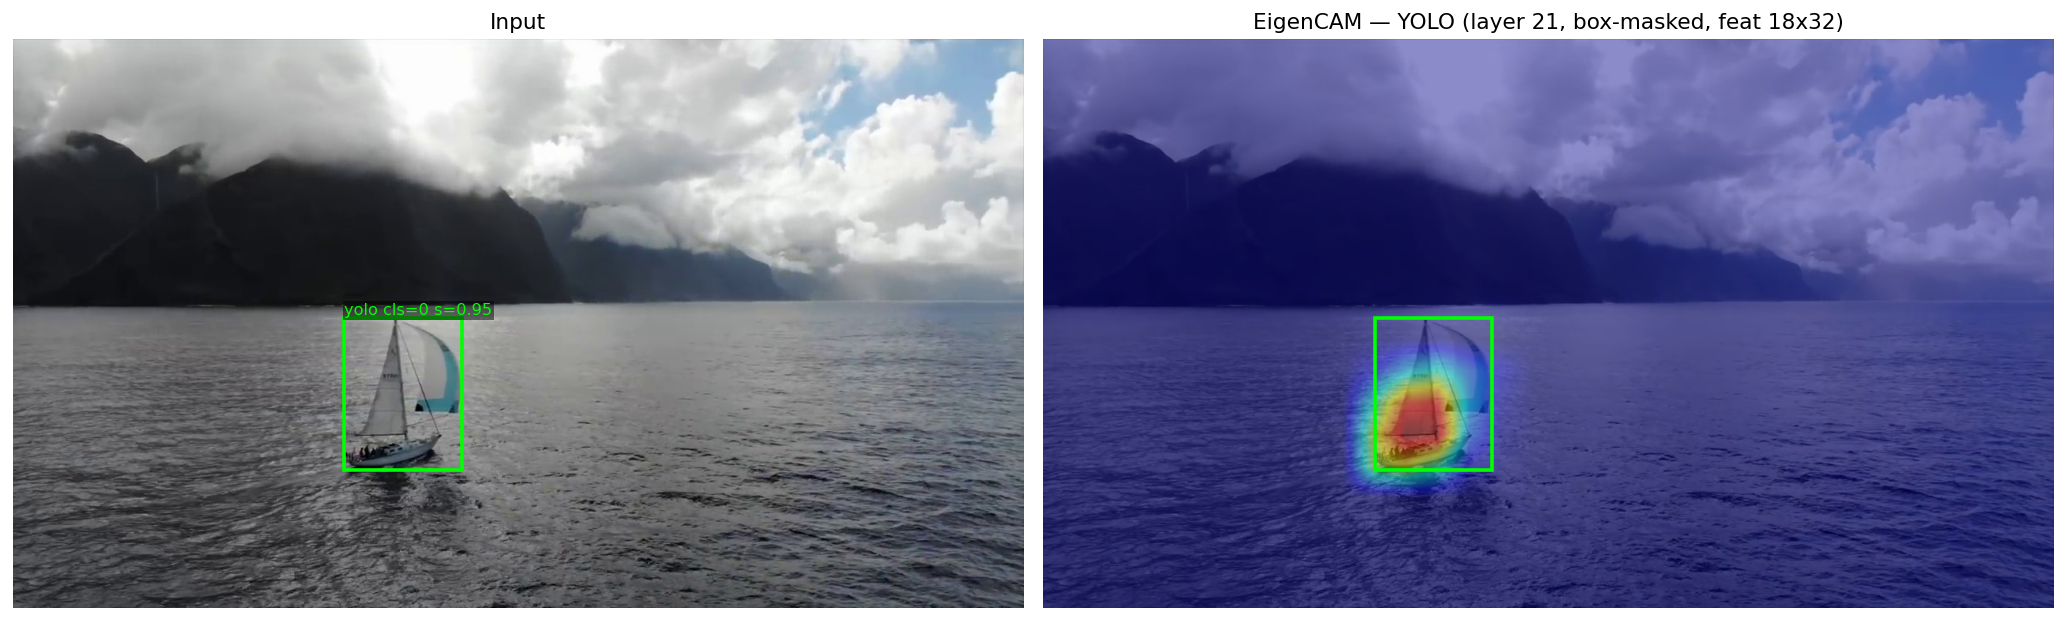
\includegraphics[width=0.85\textwidth]{xai_eigencam_yolo.png}
    \caption{EigenCAM explanation for YOLOv8.}
    \label{fig:xai_eigencam}
\end{figure}

\subsubsection{RF-DETR Attention Results}
Figure~\ref{fig:xai_rfdetr_attention} shows the RF-DETR cross-attention. The left
panel is the prediction, the middle panel is the attention of a single object
query, and the right panel aggregates the attention of several queries. A single
query concentrates on one object and roughly covers it, while the aggregated
queries line up with the outer edges of the objects in the scene. What this tells
us about the model's reliability is discussed in Section~\ref{sec:xai_discussion}.
\begin{figure}[H]
    \centering
    \includegraphics[width=\textwidth]{{xai_xattn_rfdetr__img-inhouse_seq_135_00044__sigma-15.0__topk-20__conf-0.4}.png}
    \caption{RF-DETR cross-attention. Left: prediction. Middle: a single object
    query attends to one object. Right: aggregating multiple queries highlights
    the outer edges of the objects.}
    \label{fig:xai_rfdetr_attention}
\end{figure}

\section{Discussion}

\subsection{Interpretation Of Quantitative Results}
% TODO: Accuracy, speed, class-level patterns, threshold behavior.
RF-DETR is clearly the strongest model on our test split. It leads on every
accuracy metric (34.1 mAP@50:95, 58.6 mAP@50, 81.2\% precision, 67.7\% recall),
well ahead of the two CNN baselines, which are close to each other. The error
analysis by object size supports this: RF-DETR makes fewer mistakes than the
others across the whole size range and recovers more small objects, so its lead is
not just an artefact of one metric.

Two caveats apply to the absolute numbers. First, the scores look modest in
absolute terms. For reference, the best detectors reach much higher mAP on
COCO, but this is not a fair comparison: COCO is a clean, general dataset, while
LaRS is a harder maritime setting with many tiny objects, strong class imbalance,
and residual label noise. The comparison is only meant to give a sense of scale.
Second, our cross-validation relabeling cleaned the labels using RF-DETR fold
models, so the cleaned test set is biased towards what RF-DETR detects, which
gives RF-DETR some advantage in the numbers. The gap to the other models
is large and also shows up in the qualitative live-video test, however, so we do not think
the relabeling explains it away.

A pattern shared by all models is that the dominant error is \emph{missing}
objects (predicting background) rather than confusing one class with another. This
points to label noise (missing ground-truth boxes) and small-object difficulty as
the main limiting factors, not weak classification. Faster R-CNN is the least
attractive of the three here: it is the slowest and no more accurate than YOLOv8.

\subsection{Interpretation Of Qualitative Results}
% TODO: Inference examples, false positives, false negatives, difficult scenes.
To check behaviour beyond the static test set, we ran the models on live video. A
large boat in the centre of the scene is detected by all models with high
confidence; its bounding box only becomes unstable when the background visually
``extends'' the ship's mast, so the model is unsure where the object ends. Smaller
and incoming objects are harder. A row boat and a bird that enter the frame are
eventually detected by all models, but the detections flicker because the
confidence is low, and the row boat is repeatedly switched to the boat/ship class.
RF-DETR keeps the correct class for the most frames, including for the incoming
bird; when the bird is far away it is read as a buoy, which is reasonable given how
small and featureless it looks at that distance.

The example frame in Figure~\ref{fig:inference_examples} shows the same effects
across the models. All three correctly detect the large ship in the centre, with
the box occasionally flickering when a model is unsure of its size. For the row
boat, Faster R-CNN and YOLOv8 mostly label it as a boat/ship, while RF-DETR more
often assigns the correct row-boat class. For the incoming bird, RF-DETR predicts
the animal class most reliably, YOLOv8 usually falls back to the open-world
``other'' class, and Faster R-CNN is only sometimes correct. RF-DETR is therefore
the most stable of the three, even though all of them work and all produce noisy,
flickering predictions.

These observations match the quantitative results: the models are reliable on
large, clear objects and struggle with small, ambiguous ones. They also reveal a
limitation of frame-by-frame detection: the predictions are not temporally stable.
Live deployment on a USV would benefit from temporal smoothing or tracking across
frames, which we did not explore here.

\subsection{Interpretation Of XAI Results}
\label{sec:xai_discussion}
% TODO: Compare explanation quality and model focus areas.
The RF-DETR attention maps give some insight into how the transformer reaches a
detection. A single object query concentrates its attention on one object and
roughly covers it, and when we aggregate several queries the attention lines up
with the outer edges of the objects in the scene. This suggests the model looks at
the objects themselves rather than at the surrounding water or its reflections,
which is exactly the failure mode we were worried about in a maritime setting. In
other words, when RF-DETR detects a boat, it does so because it attends to the
boat, not to the glare or the wake. We treat this as supporting evidence rather
than proof, since attention maps show where the model responds, not strictly what
caused the decision.

\subsection{Practical Relevance For Maritime Navigation}
% TODO: Deployment relevance, real-time constraints, safety implications.
For a real USV the vision system has to be both accurate and fast, and it has to
run on limited on-board hardware. Our results suggest RF-DETR is the best fit: it
is the most accurate model and still runs in real time (27 FPS), giving the best
accuracy/speed balance. YOLOv8 is the fastest (50 FPS) and is the better choice
when compute is very limited or a higher frame rate is needed; since much of its
disadvantage is tied to label quality, it could become competitive once the labels
are improved. Faster R-CNN is hard to justify here, as it is the slowest without
being more accurate.

Two further points matter for deployment. First, detecting small objects reliably
is a safety issue, since a missed buoy or swimmer is the most dangerous kind of
error, so the small-object weakness must be addressed before real use. Second,
licensing differs between the models: RF-DETR (Apache-2.0) and Faster R-CNN via
torchvision (BSD) are permissive and can be used in a closed commercial product,
whereas YOLOv8 (AGPL-3.0) would require a paid enterprise licence for that use.
This also favours RF-DETR for a commercial maritime system.

\section{Limitations}

\subsection{Dataset Limitations}
% TODO: Label noise, class imbalance, original test split lacks bbox labels.
The dataset has two main weaknesses for our task. First, the detection labels are
noisy, because they are derived from panoptic masks, and we could only partly
clean them. Second, the classes are strongly imbalanced: boat/ship dominates,
while several classes are very rare. This is especially severe in the test set,
where Float has only 4 objects, Animal 14, and Paddle board 31. The per-class
scores for these classes are therefore based on a handful of objects and should be
read as rough indicators, not reliable numbers.

\subsection{Modeling Limitations}
% TODO: Training budget, model variants, hyperparameter search limits.
We did not train any model from scratch and worked within a limited compute and
time budget. The hyperparameter search therefore ran only a modest number of
trials per model, and we did not retrain the best configurations many times. We
also covered only three detector families with one or two variants each; newer
versions (for example newer YOLO releases) and other architectures were out of
scope and would be worth revisiting once the label noise is fully resolved.

\subsection{Evaluation Limitations}
% TODO: Test split construction, metrics, qualitative analysis constraints.
We evaluate on a single test split and did not repeat training runs, so we report
no statistical significance tests and cannot rule out that part of the differences
between models comes from run-to-run variation. We also did not use nested
cross-validation, which would give a less biased estimate, because it was too
expensive for these long-training models. Most importantly, the relabeling was
done with RF-DETR, so the cleaned test labels favour RF-DETR and its measured lead
is partly self-reinforcing, even though the qualitative results suggest the lead
is real.

\subsection{XAI Limitations}
% TODO: Faithfulness, interpretability, method-specific caveats.
The explanation methods are not ground truth. Attention maps and saliency methods
show where a model responds strongly, but a bright region does not prove that the
model used that region in a causal sense. The methods also differ per model
(deformable attention for RF-DETR, CAM-based methods for the CNNs, D-RISE for
all), so comparisons across models are qualitative. We therefore use the XAI
results as supporting evidence, not as proof.

\section{Conclusion}
% TODO: Main findings and best model summary.
We benchmarked three object detectors for maritime obstacle detection on the LaRS
dataset and compared them on accuracy, speed, errors, and explainability. RF-DETR
is our recommended model: it gives the best accuracy, still runs in real time,
behaves best on live video, and has a permissive licence for real deployment.
YOLOv8 is the best option when speed or limited hardware is the priority, and it is
likely to become more competitive once the label quality is improved. Faster R-CNN
is dominated by the other two here. The main open challenge is detecting very
small objects, which all models struggle with.

Three lessons stand out from the project. Label quality matters more than we
expected and was the single biggest factor on the results. Visualising predictions
and errors, per class, per object size, and on video, was essential for
understanding what the numbers really meant. And the hyperparameter search space
should be planned carefully up front, because trial-and-error is too costly for
models that take a long time to train.

\section{Future Work}
% TODO: Vision Mamba, stronger relabeling, video/temporal cues, deployment tests.
Several directions follow from our limitations. The most important is to further
reduce the label noise, for example by using a vision-language model (VLM) to
help clean or verify the annotations, and then re-run the benchmark on cleaner
data, which would also remove the relabeling bias towards RF-DETR. To improve
small-object detection, larger models, higher input resolutions, or training
strategies aimed at small objects should be explored. For live deployment,
temporal methods such as smoothing or tracking across frames would reduce the
flickering we observed in the video. Finally, more architectures and newer model
versions, including state-space models such as Vision Mamba, could be added to
the comparison once the data quality is settled.

\clearpage
\bibliographystyle{plain}
\bibliography{references}


\begingroup
\renewcommand{\section}[2]{}
\begin{thebibliography}{9}
\setcounter{enumiv}{8}

\bibitem{petsiuk2021drise}
Vitali Petsiuk, Rajiv Jain, Varun Manjunatha, Vlad I. Morariu,
Ashutosh Mehra, Vicente Ordonez, and Kate Saenko.
\textit{Black-Box Explanation of Object Detectors via Saliency Maps}.
arXiv preprint arXiv:2006.03204, 2021.



\end{thebibliography}
\endgroup

\end{document}